\documentclass[12pt,landscape]{article}

%\usepackage{lmodern}
\usepackage{amssymb,amsmath}
\usepackage{bm}
\usepackage{graphicx}
\usepackage{microtype}
\usepackage{hyperref}
\pagestyle{empty}
\usepackage{titlesec}
\titleformat*{\section}{\LARGE\bfseries}
\titleformat*{\subsection}{\LARGE\bfseries}
\titleformat*{\subsubsection}{\LARGE\bfseries}
\setlength{\parindent}{0pt}
\setlength{\parskip}{1.2ex}
\setlength{\parindent}{0pt}
\setlength{\parskip}{1.2ex}

\setlength{\oddsidemargin}{-16mm}
\setlength{\textwidth}{260mm}
\setlength{\columnsep}{0.5in}
\setlength{\columnseprule}{1pt}
\setlength{\textheight}{202mm}
\setlength{\topmargin}{-32mm}
\setlength{\headsep}{0.25in}

\hypersetup
       {   pdfauthor = { Marco Fasondini },
           pdftitle={ foo },
           colorlinks=TRUE,
           linkcolor=black,
           citecolor=blue,
           urlcolor=blue
       }




\usepackage{upquote}
\usepackage{listings}
\usepackage{xcolor}
\lstset{
    basicstyle=\ttfamily\footnotesize,
    upquote=true,
    breaklines=true,
    breakindent=0pt,
    keepspaces=true,
    showspaces=false,
    columns=fullflexible,
    showtabs=false,
    showstringspaces=false,
    escapeinside={(*@}{@*)},
    extendedchars=true,
}
\newcommand{\HLJLt}[1]{#1}
\newcommand{\HLJLw}[1]{#1}
\newcommand{\HLJLe}[1]{#1}
\newcommand{\HLJLeB}[1]{#1}
\newcommand{\HLJLo}[1]{#1}
\newcommand{\HLJLk}[1]{\textcolor[RGB]{148,91,176}{\textbf{#1}}}
\newcommand{\HLJLkc}[1]{\textcolor[RGB]{59,151,46}{\textit{#1}}}
\newcommand{\HLJLkd}[1]{\textcolor[RGB]{214,102,97}{\textit{#1}}}
\newcommand{\HLJLkn}[1]{\textcolor[RGB]{148,91,176}{\textbf{#1}}}
\newcommand{\HLJLkp}[1]{\textcolor[RGB]{148,91,176}{\textbf{#1}}}
\newcommand{\HLJLkr}[1]{\textcolor[RGB]{148,91,176}{\textbf{#1}}}
\newcommand{\HLJLkt}[1]{\textcolor[RGB]{148,91,176}{\textbf{#1}}}
\newcommand{\HLJLn}[1]{#1}
\newcommand{\HLJLna}[1]{#1}
\newcommand{\HLJLnb}[1]{#1}
\newcommand{\HLJLnbp}[1]{#1}
\newcommand{\HLJLnc}[1]{#1}
\newcommand{\HLJLncB}[1]{#1}
\newcommand{\HLJLnd}[1]{\textcolor[RGB]{214,102,97}{#1}}
\newcommand{\HLJLne}[1]{#1}
\newcommand{\HLJLneB}[1]{#1}
\newcommand{\HLJLnf}[1]{\textcolor[RGB]{66,102,213}{#1}}
\newcommand{\HLJLnfm}[1]{\textcolor[RGB]{66,102,213}{#1}}
\newcommand{\HLJLnp}[1]{#1}
\newcommand{\HLJLnl}[1]{#1}
\newcommand{\HLJLnn}[1]{#1}
\newcommand{\HLJLno}[1]{#1}
\newcommand{\HLJLnt}[1]{#1}
\newcommand{\HLJLnv}[1]{#1}
\newcommand{\HLJLnvc}[1]{#1}
\newcommand{\HLJLnvg}[1]{#1}
\newcommand{\HLJLnvi}[1]{#1}
\newcommand{\HLJLnvm}[1]{#1}
\newcommand{\HLJLl}[1]{#1}
\newcommand{\HLJLld}[1]{\textcolor[RGB]{148,91,176}{\textit{#1}}}
\newcommand{\HLJLs}[1]{\textcolor[RGB]{201,61,57}{#1}}
\newcommand{\HLJLsa}[1]{\textcolor[RGB]{201,61,57}{#1}}
\newcommand{\HLJLsb}[1]{\textcolor[RGB]{201,61,57}{#1}}
\newcommand{\HLJLsc}[1]{\textcolor[RGB]{201,61,57}{#1}}
\newcommand{\HLJLsd}[1]{\textcolor[RGB]{201,61,57}{#1}}
\newcommand{\HLJLsdB}[1]{\textcolor[RGB]{201,61,57}{#1}}
\newcommand{\HLJLsdC}[1]{\textcolor[RGB]{201,61,57}{#1}}
\newcommand{\HLJLse}[1]{\textcolor[RGB]{59,151,46}{#1}}
\newcommand{\HLJLsh}[1]{\textcolor[RGB]{201,61,57}{#1}}
\newcommand{\HLJLsi}[1]{#1}
\newcommand{\HLJLso}[1]{\textcolor[RGB]{201,61,57}{#1}}
\newcommand{\HLJLsr}[1]{\textcolor[RGB]{201,61,57}{#1}}
\newcommand{\HLJLss}[1]{\textcolor[RGB]{201,61,57}{#1}}
\newcommand{\HLJLssB}[1]{\textcolor[RGB]{201,61,57}{#1}}
\newcommand{\HLJLnB}[1]{\textcolor[RGB]{59,151,46}{#1}}
\newcommand{\HLJLnbB}[1]{\textcolor[RGB]{59,151,46}{#1}}
\newcommand{\HLJLnfB}[1]{\textcolor[RGB]{59,151,46}{#1}}
\newcommand{\HLJLnh}[1]{\textcolor[RGB]{59,151,46}{#1}}
\newcommand{\HLJLni}[1]{\textcolor[RGB]{59,151,46}{#1}}
\newcommand{\HLJLnil}[1]{\textcolor[RGB]{59,151,46}{#1}}
\newcommand{\HLJLnoB}[1]{\textcolor[RGB]{59,151,46}{#1}}
\newcommand{\HLJLoB}[1]{\textcolor[RGB]{102,102,102}{\textbf{#1}}}
\newcommand{\HLJLow}[1]{\textcolor[RGB]{102,102,102}{\textbf{#1}}}
\newcommand{\HLJLp}[1]{#1}
\newcommand{\HLJLc}[1]{\textcolor[RGB]{153,153,119}{\textit{#1}}}
\newcommand{\HLJLch}[1]{\textcolor[RGB]{153,153,119}{\textit{#1}}}
\newcommand{\HLJLcm}[1]{\textcolor[RGB]{153,153,119}{\textit{#1}}}
\newcommand{\HLJLcp}[1]{\textcolor[RGB]{153,153,119}{\textit{#1}}}
\newcommand{\HLJLcpB}[1]{\textcolor[RGB]{153,153,119}{\textit{#1}}}
\newcommand{\HLJLcs}[1]{\textcolor[RGB]{153,153,119}{\textit{#1}}}
\newcommand{\HLJLcsB}[1]{\textcolor[RGB]{153,153,119}{\textit{#1}}}
\newcommand{\HLJLg}[1]{#1}
\newcommand{\HLJLgd}[1]{#1}
\newcommand{\HLJLge}[1]{#1}
\newcommand{\HLJLgeB}[1]{#1}
\newcommand{\HLJLgh}[1]{#1}
\newcommand{\HLJLgi}[1]{#1}
\newcommand{\HLJLgo}[1]{#1}
\newcommand{\HLJLgp}[1]{#1}
\newcommand{\HLJLgs}[1]{#1}
\newcommand{\HLJLgsB}[1]{#1}
\newcommand{\HLJLgt}[1]{#1}



\def\qqand{\qquad\hbox{and}\qquad}
\def\qqfor{\qquad\hbox{for}\qquad}
\def\qqas{\qquad\hbox{as}\qquad}
\def\half{ {1 \over 2} }
\def\D{ {\rm d} }
\def\I{ {\rm i} }
\def\E{ {\rm e} }
\def\C{ {\mathbb C} }
\def\R{ {\mathbb R} }
\def\H{ {\mathbb H} }
\def\Z{ {\mathbb Z} }
\def\CC{ {\cal C} }
\def\FF{ {\cal F} }
\def\HH{ {\cal H} }
\def\LL{ {\cal L} }
\def\vc#1{ {\mathbf #1} }
\def\bbC{ {\mathbb C} }



\def\fR{ f_{\rm R} }
\def\fL{ f_{\rm L} }

\def\qqqquad{\qquad\qquad}
\def\qqwhere{\qquad\hbox{where}\qquad}
\def\Res_#1{\underset{#1}{\rm Res}\,}
\def\sech{ {\rm sech}\, }
\def\acos{ {\rm acos}\, }
\def\asin{ {\rm asin}\, }
\def\atan{ {\rm atan}\, }
\def\Ei{ {\rm Ei}\, }
\def\upepsilon{\varepsilon}


\def\Xint#1{ \mathchoice
   {\XXint\displaystyle\textstyle{#1} }%
   {\XXint\textstyle\scriptstyle{#1} }%
   {\XXint\scriptstyle\scriptscriptstyle{#1} }%
   {\XXint\scriptscriptstyle\scriptscriptstyle{#1} }%
   \!\int}
\def\XXint#1#2#3{ {\setbox0=\hbox{$#1{#2#3}{\int}$}
     \vcenter{\hbox{$#2#3$}}\kern-.5\wd0} }
\def\ddashint{\Xint=}
\def\dashint{\Xint-}
% \def\dashint
\def\infdashint{\dashint_{-\infty}^\infty}




\def\addtab#1={#1\;&=}
\def\ccr{\\\addtab}
\def\ip<#1>{\left\langle{#1}\right\rangle}
\def\dx{\D x}
\def\dt{\D t}
\def\dz{\D z}
\def\ds{\D s}

\def\rR{ {\rm R} }
\def\rL{ {\rm L} }

\def\norm#1{\left\| #1 \right\|}

\def\pr(#1){\left({#1}\right)}
\def\br[#1]{\left[{#1}\right]}

\def\abs#1{\left|{#1}\right|}
\def\fpr(#1){\!\pr({#1})}

\def\sopmatrix#1{ \begin{pmatrix}#1\end{pmatrix} }

\def\endash{–}
\def\emdash{—}
\def\mdblksquare{\blacksquare}
\def\lgblksquare{\blacksquare}
\def\scre{\E}
\def\mapengine#1,#2.{\mapfunction{#1}\ifx\void#2\else\mapengine #2.\fi }

\def\map[#1]{\mapengine #1,\void.}

\def\mapenginesep_#1#2,#3.{\mapfunction{#2}\ifx\void#3\else#1\mapengine #3.\fi }

\def\mapsep_#1[#2]{\mapenginesep_{#1}#2,\void.}


\def\vcbr[#1]{\pr(#1)}


\def\bvect[#1,#2]{
{
\def\dots{\cdots}
\def\mapfunction##1{\ | \  ##1}
	\sopmatrix{
		 \,#1\map[#2]\,
	}
}
}



\def\vect[#1]{
{\def\dots{\ldots}
	\vcbr[{#1}]
} }

\def\vectt[#1]{
{\def\dots{\ldots}
	\vect[{#1}]^{\top}
} }

\def\Vectt[#1]{
{
\def\mapfunction##1{##1 \cr}
\def\dots{\vdots}
	\begin{pmatrix}
		\map[#1]
	\end{pmatrix}
} }

\def\addtab#1={#1\;&=}
\def\ccr{\\\addtab}

\def\questionequals{= \!\!\!\!\!\!{\scriptstyle ? \atop }\,\,\,}

\def\cent#1{\begin{center}#1\end{center} }

\lstset{
    basicstyle=\ttfamily,
	}

\begin{document}
{\LARGE
\sf
\textbf{Applied Complex Analysis (2021)}

\section{Solution Sheet 3}
\subsection{Problem 1.1}
\subsubsection{1.}
Take as an initial guess

\[
 \phi_1(z) = {\sqrt{z-1} \sqrt{z+1}  \over 2\I(1 + z^2)}
\]
This satisfies for $-1 < x < 1$

\[
\phi_1^+(x) -\phi_1^-(x) = { \sqrt{1-x^2}  \over 2(1 + x^2)} -  {- \sqrt{1-x^2}  \over 2(1 + x^2)} = {\sqrt{1 - x^2} \over 1+x^2}
\]
Further, as $z \rightarrow \infty$,

\[
\phi_1(z) \sim {z \over \I(1+ z^2)} \rightarrow 0
\]
The catch is that it has poles at $\pm \I$:


\begin{align*}
    \phi_1(z) = -{\sqrt{\I -1} \sqrt{\I+1} \over 4} { 1 \over z - \I} + O(1)  \\
    \phi_1(z) = {\sqrt{-\I -1} \sqrt{-\I+1} \over 4} { 1 \over z + \I} + O(1)
\end{align*}
Thus it follows that

\[
\phi(z) =  \phi_1(z) + {\sqrt{\I -1} \sqrt{\I+1} \over 4} { 1 \over z - \I} - {\sqrt{-\I -1} \sqrt{-\I+1} \over 4} { 1 \over z + \I}
\]
is

\begin{itemize}
\item[1. ] Analyticity: Analytic at $\pm \I$ and off $[-1,1]$


\item[2. ] Decay: $\phi(\infty) = 0$


\item[3. ] Regularity: Has weaker than pole singularities


\item[4. ] Jump: Satisfies

\end{itemize}
\[
\phi_+(x) - \phi_-(x) = {\sqrt{1-x^2} \over 1+x^2}
\]
By Plemelj II, this must be the Cauchy transform.

\emph{Demonstration} We will see experimentally that it correct. First we do a phase plot to make sure we satisfy (Analyticity):


\begin{lstlisting}
(*@\HLJLk{using}@*) (*@\HLJLn{ComplexPhasePortrait}@*)(*@\HLJLp{,}@*) (*@\HLJLn{Plots}@*)(*@\HLJLp{,}@*) (*@\HLJLn{ApproxFun}@*)(*@\HLJLp{,}@*) (*@\HLJLn{SingularIntegralEquations}@*)

(*@\HLJLnf{H}@*)(*@\HLJLp{(}@*)(*@\HLJLn{f}@*)(*@\HLJLp{)}@*) (*@\HLJLoB{=}@*) (*@\HLJLoB{-}@*)(*@\HLJLnf{hilbert}@*)(*@\HLJLp{(}@*)(*@\HLJLn{f}@*)(*@\HLJLp{)}@*)
(*@\HLJLnf{H}@*)(*@\HLJLp{(}@*)(*@\HLJLn{f}@*)(*@\HLJLp{,}@*)(*@\HLJLn{x}@*)(*@\HLJLp{)}@*) (*@\HLJLoB{=}@*) (*@\HLJLoB{-}@*)(*@\HLJLnf{hilbert}@*)(*@\HLJLp{(}@*)(*@\HLJLn{f}@*)(*@\HLJLp{,}@*)(*@\HLJLn{x}@*)(*@\HLJLp{)}@*)

(*@\HLJLn{\ensuremath{\varphi}}@*) (*@\HLJLoB{=}@*) (*@\HLJLn{z}@*) (*@\HLJLoB{->}@*) (*@\HLJLnf{sqrt}@*)(*@\HLJLp{(}@*)(*@\HLJLn{z}@*)(*@\HLJLoB{-}@*)(*@\HLJLni{1}@*)(*@\HLJLp{)}@*)(*@\HLJLnf{sqrt}@*)(*@\HLJLp{(}@*)(*@\HLJLn{z}@*)(*@\HLJLoB{+}@*)(*@\HLJLni{1}@*)(*@\HLJLp{)}@*)(*@\HLJLoB{/}@*)(*@\HLJLp{(}@*)(*@\HLJLni{2}@*)(*@\HLJLn{im}@*)(*@\HLJLoB{*}@*)(*@\HLJLp{(}@*)(*@\HLJLni{1}@*)(*@\HLJLoB{+}@*)(*@\HLJLn{z}@*)(*@\HLJLoB{{\textasciicircum}}@*)(*@\HLJLni{2}@*)(*@\HLJLp{))}@*) (*@\HLJLoB{+}@*)
        (*@\HLJLnf{sqrt}@*)(*@\HLJLp{(}@*)(*@\HLJLn{im}@*)(*@\HLJLoB{-}@*)(*@\HLJLni{1}@*)(*@\HLJLp{)}@*)(*@\HLJLnf{sqrt}@*)(*@\HLJLp{(}@*)(*@\HLJLn{im}@*)(*@\HLJLoB{+}@*)(*@\HLJLni{1}@*)(*@\HLJLp{)}@*)(*@\HLJLoB{/}@*)(*@\HLJLni{4}@*)(*@\HLJLoB{*}@*)(*@\HLJLni{1}@*)(*@\HLJLoB{/}@*)(*@\HLJLp{(}@*)(*@\HLJLn{z}@*)(*@\HLJLoB{-}@*)(*@\HLJLn{im}@*)(*@\HLJLp{)}@*) (*@\HLJLoB{-}@*)
        (*@\HLJLnf{sqrt}@*)(*@\HLJLp{(}@*)(*@\HLJLoB{-}@*)(*@\HLJLn{im}@*)(*@\HLJLoB{-}@*)(*@\HLJLni{1}@*)(*@\HLJLp{)}@*)(*@\HLJLnf{sqrt}@*)(*@\HLJLp{(}@*)(*@\HLJLoB{-}@*)(*@\HLJLn{im}@*)(*@\HLJLoB{+}@*)(*@\HLJLni{1}@*)(*@\HLJLp{)}@*)(*@\HLJLoB{/}@*)(*@\HLJLni{4}@*)(*@\HLJLoB{*}@*)(*@\HLJLni{1}@*)(*@\HLJLoB{/}@*)(*@\HLJLp{(}@*)(*@\HLJLn{z}@*)(*@\HLJLoB{+}@*)(*@\HLJLn{im}@*)(*@\HLJLp{)}@*)

(*@\HLJLnf{phaseplot}@*)(*@\HLJLp{(}@*)(*@\HLJLoB{-}@*)(*@\HLJLnfB{3..3}@*)(*@\HLJLp{,}@*) (*@\HLJLoB{-}@*)(*@\HLJLnfB{3..3}@*)(*@\HLJLp{,}@*) (*@\HLJLn{\ensuremath{\varphi}}@*)(*@\HLJLp{)}@*)
\end{lstlisting}

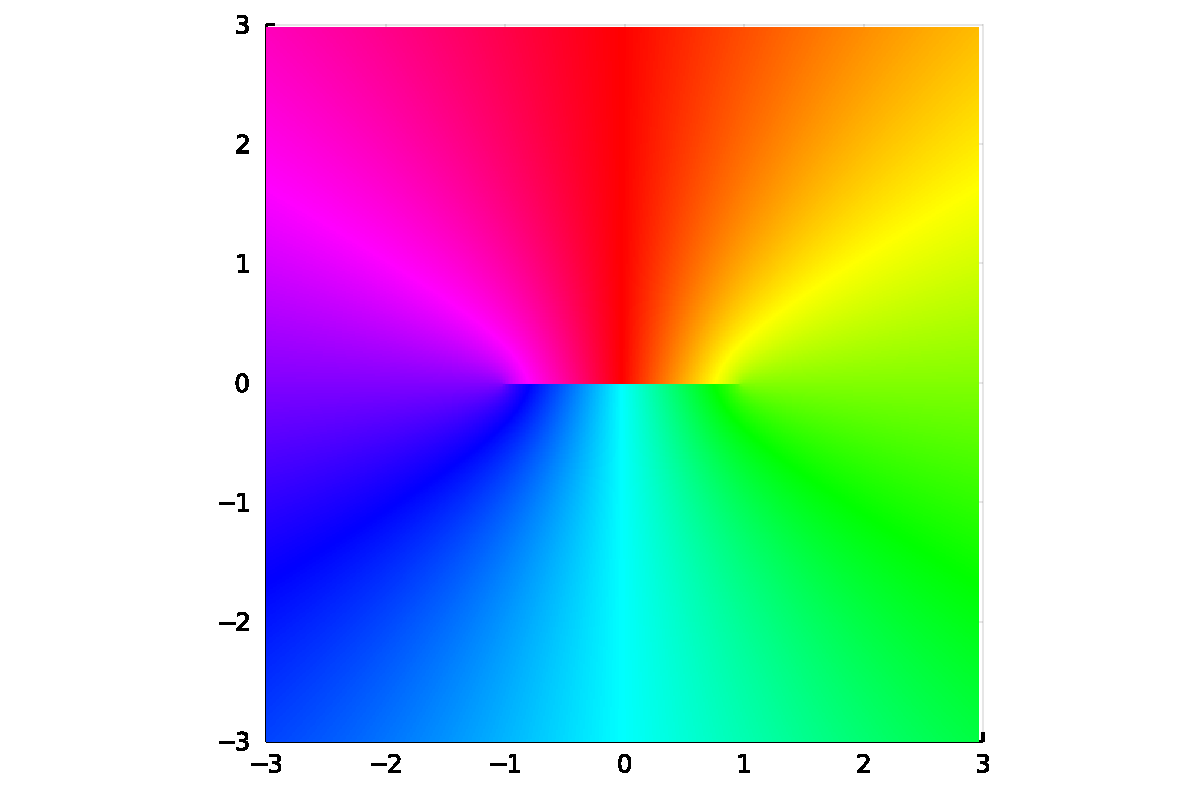
\includegraphics[width=\linewidth]{C:/Users/mfaso/OneDrive/Documents/GitHub/M3M6AppliedComplexAnalysis/output/figures/Solutions3_1_1.pdf}

We can also see from the phase plot (Regularity): we have weaker than pole singularities, otherwise we would have at least a full,counter clockwise colour wheel. We can check decay as well:


\begin{lstlisting}
(*@\HLJLnf{\ensuremath{\varphi}}@*)(*@\HLJLp{(}@*)(*@\HLJLnfB{200.0}@*)(*@\HLJLoB{+}@*)(*@\HLJLnfB{200.0}@*)(*@\HLJLn{im}@*)(*@\HLJLp{)}@*)
\end{lstlisting}

\begin{lstlisting}
0.0005177682933717976 + 0.000517765612545622im
\end{lstlisting}


Finally, we compare it numerically it to \texttt{cauchy(f, z)} which is implemented in SingularIntegralEquations.jl:


\begin{lstlisting}
(*@\HLJLn{x}@*) (*@\HLJLoB{=}@*) (*@\HLJLnf{Fun}@*)(*@\HLJLp{()}@*)
(*@\HLJLnf{\ensuremath{\varphi}}@*)(*@\HLJLp{(}@*)(*@\HLJLnfB{2.0}@*)(*@\HLJLoB{+}@*)(*@\HLJLnfB{2.0}@*)(*@\HLJLn{im}@*)(*@\HLJLp{),}@*)(*@\HLJLnf{cauchy}@*)(*@\HLJLp{(}@*)(*@\HLJLnf{sqrt}@*)(*@\HLJLp{(}@*)(*@\HLJLni{1}@*)(*@\HLJLoB{-}@*)(*@\HLJLn{x}@*)(*@\HLJLoB{{\textasciicircum}}@*)(*@\HLJLni{2}@*)(*@\HLJLp{)}@*)(*@\HLJLoB{/}@*)(*@\HLJLp{(}@*)(*@\HLJLni{1}@*)(*@\HLJLoB{+}@*)(*@\HLJLn{x}@*)(*@\HLJLoB{{\textasciicircum}}@*)(*@\HLJLni{2}@*)(*@\HLJLp{),}@*) (*@\HLJLnfB{2.0}@*)(*@\HLJLoB{+}@*)(*@\HLJLnfB{2.0}@*)(*@\HLJLn{im}@*)(*@\HLJLp{)}@*)
\end{lstlisting}

\begin{lstlisting}
(0.05303535516221752 + 0.05036581190871381im, 0.05303535516221748 + 0.05036
581190871378im)
\end{lstlisting}


\subsubsection{2.}
Recall that

\[
\psi(z) = {\log(z-1) - \log(z+1)  \over 2 \pi \I}
\]
satisfies

\[
\psi_+(x) - \psi_-(x) = 1
\]
Therefore, consider

\[
\phi_1(z) = {\psi(z) \over 2 + z}
\]
This has the right jump, but has an extra pole at $z = -2$: for $x < -1$ we have

\[
\phi_1(x) = {\log_+(x-1) - \log_+(x+1)  \over 2 \pi \I} {1 \over 2 + x} =
   {\log(1-x) - \log(-1-x)  \over 2 \pi \I} {1 \over 2 + x}
\]
hence we arrive at the solution

\[
\phi_1(z) - {\log 3 \over 2 \pi \I (2+z)}
\]
We can verify that $\phi_1(\infty) = 0$.


\begin{lstlisting}
(*@\HLJLn{\ensuremath{\varphi}}@*) (*@\HLJLoB{=}@*)  (*@\HLJLn{z}@*) (*@\HLJLoB{->}@*) (*@\HLJLp{(}@*)(*@\HLJLnf{log}@*)(*@\HLJLp{(}@*)(*@\HLJLn{z}@*)(*@\HLJLoB{-}@*)(*@\HLJLni{1}@*)(*@\HLJLp{)}@*)(*@\HLJLoB{-}@*)(*@\HLJLnf{log}@*)(*@\HLJLp{(}@*)(*@\HLJLn{z}@*)(*@\HLJLoB{+}@*)(*@\HLJLni{1}@*)(*@\HLJLp{))}@*) (*@\HLJLoB{/}@*) (*@\HLJLp{((}@*)(*@\HLJLni{2}@*)(*@\HLJLn{\ensuremath{\pi}}@*)(*@\HLJLoB{*}@*)(*@\HLJLn{im}@*)(*@\HLJLp{)}@*)(*@\HLJLoB{*}@*)(*@\HLJLp{(}@*)(*@\HLJLni{2}@*)(*@\HLJLoB{+}@*)(*@\HLJLn{z}@*)(*@\HLJLp{))}@*) (*@\HLJLoB{-}@*) (*@\HLJLnf{log}@*)(*@\HLJLp{(}@*)(*@\HLJLni{3}@*)(*@\HLJLp{)}@*)(*@\HLJLoB{/}@*)(*@\HLJLp{(}@*)(*@\HLJLni{2}@*)(*@\HLJLn{\ensuremath{\pi}}@*)(*@\HLJLoB{*}@*)(*@\HLJLn{im}@*)(*@\HLJLoB{*}@*)(*@\HLJLp{(}@*)(*@\HLJLni{2}@*)(*@\HLJLoB{+}@*)(*@\HLJLn{z}@*)(*@\HLJLp{))}@*)

(*@\HLJLnf{phaseplot}@*)(*@\HLJLp{(}@*)(*@\HLJLoB{-}@*)(*@\HLJLnfB{3..3}@*)(*@\HLJLp{,}@*) (*@\HLJLoB{-}@*)(*@\HLJLnfB{3..3}@*)(*@\HLJLp{,}@*) (*@\HLJLn{\ensuremath{\varphi}}@*)(*@\HLJLp{)}@*)
\end{lstlisting}

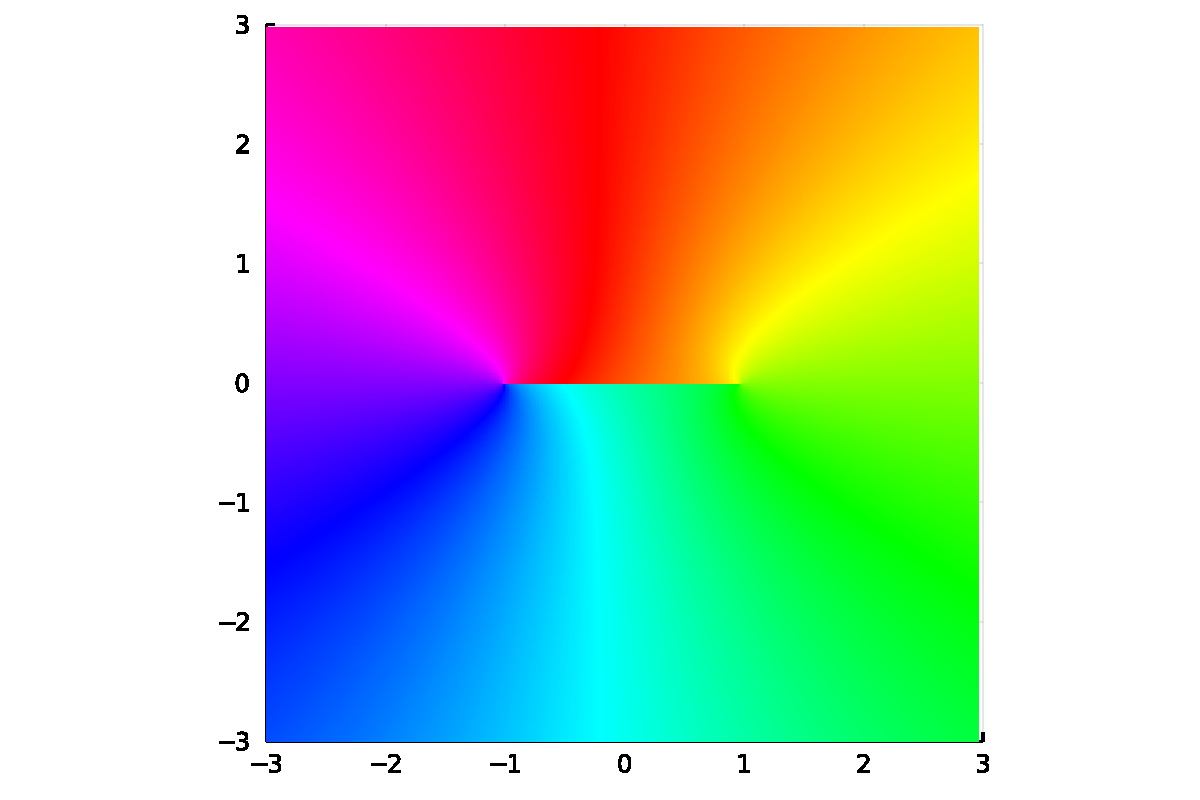
\includegraphics[width=\linewidth]{C:/Users/mfaso/OneDrive/Documents/GitHub/M3M6AppliedComplexAnalysis/output/figures/Solutions3_4_1.pdf}

\subsubsection{3.}
We first calculate the Cauchy transform of $f(x) = x/\sqrt{1-x^2}$:

\[
\phi(z) = {\I z  \over 2 \sqrt{z -1} \sqrt{z+1}} - {\I \over 2}
\]
This vanishes at $\infty$ and has the correct jump. We then have

\[
\I{\cal H}f(x) = \phi^+(x) + \phi^-(x) = -\I
\]
This implies that (note the sign)

\[
\dashint_{-1}^1 {t \over (t-x) \sqrt{1-t^2}} \dt = -\pi \HH f(x) = \pi
\]

\begin{lstlisting}
(*@\HLJLn{f}@*) (*@\HLJLoB{=}@*) (*@\HLJLn{x}@*)(*@\HLJLoB{/}@*)(*@\HLJLnf{sqrt}@*)(*@\HLJLp{(}@*)(*@\HLJLni{1}@*)(*@\HLJLoB{-}@*)(*@\HLJLn{x}@*)(*@\HLJLoB{{\textasciicircum}}@*)(*@\HLJLni{2}@*)(*@\HLJLp{)}@*)
(*@\HLJLoB{-}@*)(*@\HLJLn{\ensuremath{\pi}}@*)(*@\HLJLoB{*}@*)(*@\HLJLnf{H}@*)(*@\HLJLp{(}@*)(*@\HLJLn{f}@*)(*@\HLJLp{,}@*) (*@\HLJLnfB{0.1}@*)(*@\HLJLp{)}@*)
\end{lstlisting}

\begin{lstlisting}
3.141592653589793
\end{lstlisting}


\subsection{Problem 1.2}
\subsubsection{1.2.1}
From Problem 1.1 part 3, we have a solution:

\[
\phi(z) = -{ z  \over 2 \sqrt{z -1} \sqrt{z+1}} + {1 \over 2}
\]
All other solutions are then of the form:

\[
\phi(z) + {C \over \sqrt{z-1} \sqrt{z+1}}
\]

\begin{lstlisting}
(*@\HLJLn{C}@*) (*@\HLJLoB{=}@*) (*@\HLJLnf{randn}@*)(*@\HLJLp{()}@*)
(*@\HLJLn{\ensuremath{\varphi}}@*) (*@\HLJLoB{=}@*) (*@\HLJLn{z}@*) (*@\HLJLoB{->}@*) (*@\HLJLoB{-}@*)(*@\HLJLn{z}@*)(*@\HLJLoB{/}@*)(*@\HLJLp{(}@*)(*@\HLJLni{2}@*)(*@\HLJLoB{*}@*)(*@\HLJLnf{sqrt}@*)(*@\HLJLp{(}@*)(*@\HLJLn{z}@*)(*@\HLJLoB{-}@*)(*@\HLJLni{1}@*)(*@\HLJLp{)}@*)(*@\HLJLoB{*}@*)(*@\HLJLnf{sqrt}@*)(*@\HLJLp{(}@*)(*@\HLJLn{z}@*)(*@\HLJLoB{+}@*)(*@\HLJLni{1}@*)(*@\HLJLp{))}@*)(*@\HLJLoB{+}@*)(*@\HLJLni{1}@*)(*@\HLJLoB{/}@*)(*@\HLJLni{2}@*) (*@\HLJLoB{+}@*) (*@\HLJLn{C}@*)(*@\HLJLoB{/}@*)(*@\HLJLp{(}@*)(*@\HLJLnf{sqrt}@*)(*@\HLJLp{(}@*)(*@\HLJLn{z}@*)(*@\HLJLoB{-}@*)(*@\HLJLni{1}@*)(*@\HLJLp{)}@*)(*@\HLJLoB{*}@*)(*@\HLJLnf{sqrt}@*)(*@\HLJLp{(}@*)(*@\HLJLn{z}@*)(*@\HLJLoB{+}@*)(*@\HLJLni{1}@*)(*@\HLJLp{))}@*)
(*@\HLJLnf{\ensuremath{\varphi}}@*)(*@\HLJLp{(}@*)(*@\HLJLnfB{0.1}@*)(*@\HLJLoB{+}@*)(*@\HLJLnfB{0.0}@*)(*@\HLJLn{im}@*)(*@\HLJLp{)}@*)(*@\HLJLoB{+}@*)(*@\HLJLnf{\ensuremath{\varphi}}@*)(*@\HLJLp{(}@*)(*@\HLJLnfB{0.1}@*)(*@\HLJLoB{-}@*)(*@\HLJLnfB{0.0}@*)(*@\HLJLn{im}@*)(*@\HLJLp{),}@*) (*@\HLJLnf{\ensuremath{\varphi}}@*)(*@\HLJLp{(}@*)(*@\HLJLnfB{1E8}@*)(*@\HLJLp{)}@*)
\end{lstlisting}

\begin{lstlisting}
(1.0 + 0.0im, -1.782207108835652e-8)
\end{lstlisting}


\subsubsection{1.2.2}
\[
\psi(z) = -2\phi(z) + 1 = { z  \over  \sqrt{z -1} \sqrt{z+1}}
\]
satisfies

\[
\psi_+(x) + \psi_-(x) = 0, \qquad \psi(\infty) = 1
\]

\begin{lstlisting}
(*@\HLJLn{C}@*) (*@\HLJLoB{=}@*) (*@\HLJLnf{randn}@*)(*@\HLJLp{()}@*)
(*@\HLJLn{\ensuremath{\varphi}}@*) (*@\HLJLoB{=}@*) (*@\HLJLn{z}@*) (*@\HLJLoB{->}@*) (*@\HLJLn{z}@*)(*@\HLJLoB{/}@*)(*@\HLJLp{(}@*)(*@\HLJLnf{sqrt}@*)(*@\HLJLp{(}@*)(*@\HLJLn{z}@*)(*@\HLJLoB{-}@*)(*@\HLJLni{1}@*)(*@\HLJLp{)}@*)(*@\HLJLoB{*}@*)(*@\HLJLnf{sqrt}@*)(*@\HLJLp{(}@*)(*@\HLJLn{z}@*)(*@\HLJLoB{+}@*)(*@\HLJLni{1}@*)(*@\HLJLp{))}@*) (*@\HLJLoB{+}@*) (*@\HLJLn{C}@*)(*@\HLJLoB{/}@*)(*@\HLJLp{(}@*)(*@\HLJLnf{sqrt}@*)(*@\HLJLp{(}@*)(*@\HLJLn{z}@*)(*@\HLJLoB{-}@*)(*@\HLJLni{1}@*)(*@\HLJLp{)}@*)(*@\HLJLoB{*}@*)(*@\HLJLnf{sqrt}@*)(*@\HLJLp{(}@*)(*@\HLJLn{z}@*)(*@\HLJLoB{+}@*)(*@\HLJLni{1}@*)(*@\HLJLp{))}@*)

(*@\HLJLnf{\ensuremath{\varphi}}@*)(*@\HLJLp{(}@*)(*@\HLJLnfB{0.1}@*)(*@\HLJLoB{+}@*)(*@\HLJLnfB{0.0}@*)(*@\HLJLn{im}@*)(*@\HLJLp{)}@*)(*@\HLJLoB{+}@*)(*@\HLJLnf{\ensuremath{\varphi}}@*)(*@\HLJLp{(}@*)(*@\HLJLnfB{0.1}@*)(*@\HLJLoB{-}@*)(*@\HLJLnfB{0.0}@*)(*@\HLJLn{im}@*)(*@\HLJLp{),}@*)(*@\HLJLnf{\ensuremath{\varphi}}@*)(*@\HLJLp{(}@*)(*@\HLJLnfB{1E9}@*)(*@\HLJLp{)}@*)
\end{lstlisting}

\begin{lstlisting}
(0.0 + 0.0im, 0.9999999993222088)
\end{lstlisting}


\subsubsection{1.2.3}
For $f(x) = \sqrt{1-x^2}$, we use the formula

\[
\phi(z) = {\I \over \sqrt{z - 1} \sqrt{z+1}} \CC[\sqrt{1-\diamond^2} f](z) + {C \over \sqrt{z-1}\sqrt{z+1}}  = {\I \over \sqrt{z - 1} \sqrt{z+1}} \CC[1-\diamond^2](z) + {C \over \sqrt{z-1}\sqrt{z+1}}
\]
We already know $\CC1(z)$, and we can deduce $\CC[\diamond^2]$ as follows: try

\[
\phi_1(z) = z^2 \CC1(z) = z^2 {\log(z-1) - \log(z+1) \over 2 \pi \I}
\]
this has the right jump, but blows up at $\infty$ like:

\[
x^2 (\log(x-1) - \log(x+1)) = x^2 (\log(1-1/x)  - \log(1+1/x) )
= -2 x + O(x^{-1})
\]
using

\[
\log z = (z-1) - {1\over 2}(z-1)^2 + O(z-1)^3
\]
Thus we have

\[
\CC[\diamond^2](z) = {z^2 (\log(z-1) - \log(z+1)) + 2 z \over 2 \pi \I}
\]
and

\[
\phi(z) = {\I \over \sqrt{z - 1} \sqrt{z+1}} {(1-z^2)(\log(z-1) - \log(z+1)) - 2 z \over 2 \pi \I}  + {C \over \sqrt{z-1}\sqrt{z+1}}
\]
\emph{Demonstration} Here we see that the Cauchy transform of $x^2$ has the correct formula:


\begin{lstlisting}
(*@\HLJLn{z}@*) (*@\HLJLoB{=}@*) (*@\HLJLnfB{2.0}@*)(*@\HLJLoB{+}@*)(*@\HLJLnfB{2.0}@*)(*@\HLJLn{im}@*)
(*@\HLJLnf{cauchy}@*)(*@\HLJLp{(}@*)(*@\HLJLn{x}@*)(*@\HLJLoB{{\textasciicircum}}@*)(*@\HLJLni{2}@*)(*@\HLJLp{,}@*) (*@\HLJLn{z}@*)(*@\HLJLp{),(}@*)(*@\HLJLn{z}@*)(*@\HLJLoB{{\textasciicircum}}@*)(*@\HLJLni{2}@*)(*@\HLJLoB{*}@*)(*@\HLJLp{(}@*)(*@\HLJLnf{log}@*)(*@\HLJLp{(}@*)(*@\HLJLn{z}@*)(*@\HLJLoB{-}@*)(*@\HLJLni{1}@*)(*@\HLJLp{)}@*)(*@\HLJLoB{-}@*)(*@\HLJLnf{log}@*)(*@\HLJLp{(}@*)(*@\HLJLn{z}@*)(*@\HLJLoB{+}@*)(*@\HLJLni{1}@*)(*@\HLJLp{))}@*)(*@\HLJLoB{+}@*)(*@\HLJLni{2}@*)(*@\HLJLn{z}@*)(*@\HLJLp{)}@*)(*@\HLJLoB{/}@*)(*@\HLJLp{(}@*)(*@\HLJLni{2}@*)(*@\HLJLn{\ensuremath{\pi}}@*)(*@\HLJLoB{*}@*)(*@\HLJLn{im}@*)(*@\HLJLp{)}@*)
\end{lstlisting}

\begin{lstlisting}
(0.0283222937395961 + 0.024377589786690298im, 0.028322293739596032 + 0.0243
7758978669024im)
\end{lstlisting}


We now see that $\phi$ has the right jumps:


\begin{lstlisting}
(*@\HLJLn{C}@*) (*@\HLJLoB{=}@*) (*@\HLJLnf{randn}@*)(*@\HLJLp{()}@*)
(*@\HLJLn{\ensuremath{\varphi}}@*) (*@\HLJLoB{=}@*) (*@\HLJLn{z}@*) (*@\HLJLoB{->}@*) (*@\HLJLn{im}@*)(*@\HLJLoB{/}@*)(*@\HLJLp{(}@*)(*@\HLJLnf{sqrt}@*)(*@\HLJLp{(}@*)(*@\HLJLn{z}@*)(*@\HLJLoB{-}@*)(*@\HLJLni{1}@*)(*@\HLJLp{)}@*)(*@\HLJLoB{*}@*)(*@\HLJLnf{sqrt}@*)(*@\HLJLp{(}@*)(*@\HLJLn{z}@*)(*@\HLJLoB{+}@*)(*@\HLJLni{1}@*)(*@\HLJLp{))}@*) (*@\HLJLoB{*}@*) (*@\HLJLp{((}@*)(*@\HLJLni{1}@*)(*@\HLJLoB{-}@*)(*@\HLJLn{z}@*)(*@\HLJLoB{{\textasciicircum}}@*)(*@\HLJLni{2}@*)(*@\HLJLp{)}@*)(*@\HLJLoB{*}@*)(*@\HLJLp{(}@*)(*@\HLJLnf{log}@*)(*@\HLJLp{(}@*)(*@\HLJLn{z}@*)(*@\HLJLoB{-}@*)(*@\HLJLni{1}@*)(*@\HLJLp{)}@*)(*@\HLJLoB{-}@*)(*@\HLJLnf{log}@*)(*@\HLJLp{(}@*)(*@\HLJLn{z}@*)(*@\HLJLoB{+}@*)(*@\HLJLni{1}@*)(*@\HLJLp{))}@*)(*@\HLJLoB{-}@*)(*@\HLJLni{2}@*)(*@\HLJLn{z}@*)(*@\HLJLp{)}@*)(*@\HLJLoB{/}@*)(*@\HLJLp{(}@*)(*@\HLJLni{2}@*)(*@\HLJLn{\ensuremath{\pi}}@*)(*@\HLJLoB{*}@*)(*@\HLJLn{im}@*)(*@\HLJLp{)}@*) (*@\HLJLoB{+}@*) (*@\HLJLn{C}@*)(*@\HLJLoB{/}@*)(*@\HLJLp{(}@*)(*@\HLJLnf{sqrt}@*)(*@\HLJLp{(}@*)(*@\HLJLn{z}@*)(*@\HLJLoB{-}@*)(*@\HLJLni{1}@*)(*@\HLJLp{)}@*)(*@\HLJLnf{sqrt}@*)(*@\HLJLp{(}@*)(*@\HLJLn{z}@*)(*@\HLJLoB{+}@*)(*@\HLJLni{1}@*)(*@\HLJLp{))}@*)

(*@\HLJLnf{\ensuremath{\varphi}}@*)(*@\HLJLp{(}@*)(*@\HLJLnfB{0.1}@*)(*@\HLJLoB{+}@*)(*@\HLJLnfB{0.0}@*)(*@\HLJLn{im}@*)(*@\HLJLp{)}@*) (*@\HLJLoB{+}@*) (*@\HLJLnf{\ensuremath{\varphi}}@*)(*@\HLJLp{(}@*)(*@\HLJLnfB{0.1}@*)(*@\HLJLoB{-}@*)(*@\HLJLnfB{0.0}@*)(*@\HLJLn{im}@*)(*@\HLJLp{)}@*) (*@\HLJLoB{-}@*) (*@\HLJLnf{sqrt}@*)(*@\HLJLp{(}@*)(*@\HLJLni{1}@*)(*@\HLJLoB{-}@*)(*@\HLJLnfB{0.1}@*)(*@\HLJLoB{{\textasciicircum}}@*)(*@\HLJLni{2}@*)(*@\HLJLp{)}@*)
\end{lstlisting}

\begin{lstlisting}
1.1102230246251565e-16 + 0.0im
\end{lstlisting}


Finally, it vanishes at infinity:


\begin{lstlisting}
(*@\HLJLnf{\ensuremath{\varphi}}@*)(*@\HLJLp{(}@*)(*@\HLJLnfB{1E5}@*)(*@\HLJLp{)}@*)
\end{lstlisting}

\begin{lstlisting}
-6.764623255449203e-7 - 0.0im
\end{lstlisting}


\subsubsection{1.2.4}
Let $f(x) = {1 \over 1+x^2}$. From Problem 1.1 part 1 we know

\[
\CC\left[{\sqrt{1-\diamond^2}\over 1 + \diamond^2}\right] (z) = {\sqrt{z-1} \sqrt{z+1}  \over 2\I(1 + z^2)}  + {\sqrt{\I -1} \sqrt{\I+1} \over 4} { 1 \over z - \I} - {\sqrt{-\I -1} \sqrt{-\I+1} \over 4} { 1 \over z + \I}
\]
hence from the solution formula we have

\[
\phi(z) = {1  \over 2(1 + z^2)}  + {\sqrt{\I -1} \sqrt{\I+1} \I \over 4\sqrt{z-1} \sqrt{z+1}} { 1 \over z - \I} - {\sqrt{-\I -1} \sqrt{-\I+1} \I \over 4\sqrt{z-1} \sqrt{z+1}} { 1 \over z + \I} + {C \over \sqrt{z-1} \sqrt{z+1}}
\]
But we want something stronger: that $\phi(z) = O(z^{-2})$. To accomplish this, we need to choose $C$.  Fortunately, I made the problem easy as every term apart from the last one is already $O(z^{-2})$, so choose $C = 0$:


\begin{lstlisting}
(*@\HLJLn{\ensuremath{\varphi}}@*) (*@\HLJLoB{=}@*) (*@\HLJLn{z}@*) (*@\HLJLoB{->}@*) (*@\HLJLni{1}@*)(*@\HLJLoB{/}@*)(*@\HLJLp{(}@*)(*@\HLJLni{2}@*)(*@\HLJLoB{*}@*)(*@\HLJLp{(}@*)(*@\HLJLni{1}@*)(*@\HLJLoB{+}@*)(*@\HLJLn{z}@*)(*@\HLJLoB{{\textasciicircum}}@*)(*@\HLJLni{2}@*)(*@\HLJLp{))}@*) (*@\HLJLoB{+}@*)
        (*@\HLJLnf{sqrt}@*)(*@\HLJLp{(}@*)(*@\HLJLn{im}@*)(*@\HLJLoB{-}@*)(*@\HLJLni{1}@*)(*@\HLJLp{)}@*)(*@\HLJLnf{sqrt}@*)(*@\HLJLp{(}@*)(*@\HLJLn{im}@*)(*@\HLJLoB{+}@*)(*@\HLJLni{1}@*)(*@\HLJLp{)}@*)(*@\HLJLoB{*}@*)(*@\HLJLn{im}@*)(*@\HLJLoB{/}@*)(*@\HLJLp{(}@*)(*@\HLJLni{4}@*)(*@\HLJLnf{sqrt}@*)(*@\HLJLp{(}@*)(*@\HLJLn{z}@*)(*@\HLJLoB{-}@*)(*@\HLJLni{1}@*)(*@\HLJLp{)}@*)(*@\HLJLnf{sqrt}@*)(*@\HLJLp{(}@*)(*@\HLJLn{z}@*)(*@\HLJLoB{+}@*)(*@\HLJLni{1}@*)(*@\HLJLp{))}@*)(*@\HLJLoB{*}@*)(*@\HLJLni{1}@*)(*@\HLJLoB{/}@*)(*@\HLJLp{(}@*)(*@\HLJLn{z}@*)(*@\HLJLoB{-}@*)(*@\HLJLn{im}@*)(*@\HLJLp{)}@*) (*@\HLJLoB{-}@*)
        (*@\HLJLnf{sqrt}@*)(*@\HLJLp{(}@*)(*@\HLJLoB{-}@*)(*@\HLJLn{im}@*)(*@\HLJLoB{-}@*)(*@\HLJLni{1}@*)(*@\HLJLp{)}@*)(*@\HLJLnf{sqrt}@*)(*@\HLJLp{(}@*)(*@\HLJLoB{-}@*)(*@\HLJLn{im}@*)(*@\HLJLoB{+}@*)(*@\HLJLni{1}@*)(*@\HLJLp{)}@*)(*@\HLJLoB{*}@*)(*@\HLJLn{im}@*)(*@\HLJLoB{/}@*)(*@\HLJLp{(}@*)(*@\HLJLni{4}@*)(*@\HLJLnf{sqrt}@*)(*@\HLJLp{(}@*)(*@\HLJLn{z}@*)(*@\HLJLoB{-}@*)(*@\HLJLni{1}@*)(*@\HLJLp{)}@*)(*@\HLJLnf{sqrt}@*)(*@\HLJLp{(}@*)(*@\HLJLn{z}@*)(*@\HLJLoB{+}@*)(*@\HLJLni{1}@*)(*@\HLJLp{))}@*)(*@\HLJLoB{*}@*)(*@\HLJLni{1}@*)(*@\HLJLoB{/}@*)(*@\HLJLp{(}@*)(*@\HLJLn{z}@*)(*@\HLJLoB{+}@*)(*@\HLJLn{im}@*)(*@\HLJLp{)}@*)

(*@\HLJLnf{\ensuremath{\varphi}}@*)(*@\HLJLp{(}@*)(*@\HLJLnfB{1E5}@*)(*@\HLJLp{)}@*)(*@\HLJLoB{*}@*)(*@\HLJLnfB{1E5}@*)
\end{lstlisting}

\begin{lstlisting}
-2.071067812011923e-6 + 0.0im
\end{lstlisting}


We see also that it has the right jump:


\begin{lstlisting}
(*@\HLJLnf{\ensuremath{\varphi}}@*)(*@\HLJLp{(}@*)(*@\HLJLnfB{0.1}@*)(*@\HLJLoB{+}@*)(*@\HLJLnfB{0.0}@*)(*@\HLJLn{im}@*)(*@\HLJLp{)}@*) (*@\HLJLoB{+}@*) (*@\HLJLnf{\ensuremath{\varphi}}@*)(*@\HLJLp{(}@*)(*@\HLJLnfB{0.1}@*)(*@\HLJLoB{-}@*)(*@\HLJLnfB{0.0}@*)(*@\HLJLn{im}@*)(*@\HLJLp{),}@*)(*@\HLJLni{1}@*)(*@\HLJLoB{/}@*)(*@\HLJLp{(}@*)(*@\HLJLni{1}@*)(*@\HLJLoB{+}@*)(*@\HLJLnfB{0.1}@*)(*@\HLJLoB{{\textasciicircum}}@*)(*@\HLJLni{2}@*)(*@\HLJLp{)}@*)
\end{lstlisting}

\begin{lstlisting}
(0.9900990099009901 + 0.0im, 0.9900990099009901)
\end{lstlisting}


\subsection{Problem 1.3}
\begin{itemize}
\item[1. ] From the Hilbert formula, we know that the general solution of $\HH u = f$ is

\end{itemize}
\[
    u(x) =  {-1 \over \sqrt{1 - x^2}}\HH \left[{ f(\diamond)  \sqrt{1-\diamond^2} }\right](x)  - {C \over \sqrt{1-x^2}}
\]
Plugging in $f(x) = x/\sqrt{1-x^2}$ means we need to calculate

\[
\HH \left[{\diamond}\right](x)
\]
We do so by first finding the Cauchy transform. Consider

\[
\phi_1(z) = z \CC 1(z) = z {\log(z-1) - \log(z+1) \over 2 \pi \I}
\]
This has the right jump:

\[
\phi_1^+(x) - \phi_1^-(x) = x
\]
but doesn't decay at $\infty$:


\begin{align*}
x {\log(x-1) - \log(x+1) \over 2 \pi \I} = x {\log x + \log(1-1/x) - \log x -\log(1+1/x) \over 2 \pi \I} \\
= -x { 2 \over x 2 \pi \I}  = -{1 \over \I \pi}
\end{align*}
But this means that

\[
\phi(z) = \phi_1(z) + {1 \over \I \pi} = z {\log(z-1) - \log(z+1) \over 2 \pi \I}  + {1 \over \I \pi}
\]
Decays and has the right jump, hence is $\CC[\diamond](z)$.


\begin{lstlisting}
(*@\HLJLn{t}@*) (*@\HLJLoB{=}@*) (*@\HLJLnf{Fun}@*)(*@\HLJLp{()}@*)
(*@\HLJLn{z}@*) (*@\HLJLoB{=}@*) (*@\HLJLnfB{2.0}@*)(*@\HLJLoB{+}@*)(*@\HLJLnfB{2.0}@*)(*@\HLJLn{im}@*)
(*@\HLJLnf{cauchy}@*)(*@\HLJLp{(}@*)(*@\HLJLn{t}@*)(*@\HLJLp{,}@*) (*@\HLJLn{z}@*)(*@\HLJLp{),}@*) (*@\HLJLn{z}@*)(*@\HLJLoB{*}@*)(*@\HLJLp{(}@*)(*@\HLJLnf{log}@*)(*@\HLJLp{(}@*)(*@\HLJLn{z}@*)(*@\HLJLoB{-}@*)(*@\HLJLni{1}@*)(*@\HLJLp{)}@*)(*@\HLJLoB{-}@*)(*@\HLJLnf{log}@*)(*@\HLJLp{(}@*)(*@\HLJLn{z}@*)(*@\HLJLoB{+}@*)(*@\HLJLni{1}@*)(*@\HLJLp{))}@*)(*@\HLJLoB{/}@*)(*@\HLJLp{(}@*)(*@\HLJLni{2}@*)(*@\HLJLn{\ensuremath{\pi}}@*)(*@\HLJLoB{*}@*)(*@\HLJLn{im}@*)(*@\HLJLp{)}@*) (*@\HLJLoB{+}@*) (*@\HLJLni{1}@*)(*@\HLJLoB{/}@*)(*@\HLJLp{(}@*)(*@\HLJLn{im}@*)(*@\HLJLoB{*}@*)(*@\HLJLn{\ensuremath{\pi}}@*)(*@\HLJLp{)}@*)
\end{lstlisting}

\begin{lstlisting}
(0.013174970881571602 - 0.0009861759882264494im, 0.013174970881571569 - 0.0
009861759882264232im)
\end{lstlisting}


Therefore, we have

\[
\HH[\diamond](x) = -\I (\CC^+ + \CC^-) \diamond(x) = -x {\log(1-x) - \log(1+x) \over \pi} -{2 \over \pi}
\]

\begin{lstlisting}
(*@\HLJLn{x}@*) (*@\HLJLoB{=}@*) (*@\HLJLnfB{0.1}@*)
(*@\HLJLnf{H}@*)(*@\HLJLp{(}@*)(*@\HLJLn{t}@*)(*@\HLJLp{,}@*)(*@\HLJLn{x}@*)(*@\HLJLp{),}@*) (*@\HLJLoB{-}@*)(*@\HLJLn{x}@*)(*@\HLJLoB{*}@*)(*@\HLJLp{(}@*)(*@\HLJLnf{log}@*)(*@\HLJLp{(}@*)(*@\HLJLni{1}@*)(*@\HLJLoB{-}@*)(*@\HLJLn{x}@*)(*@\HLJLp{)}@*)(*@\HLJLoB{-}@*)(*@\HLJLnf{log}@*)(*@\HLJLp{(}@*)(*@\HLJLni{1}@*)(*@\HLJLoB{+}@*)(*@\HLJLn{x}@*)(*@\HLJLp{))}@*)(*@\HLJLoB{/}@*)(*@\HLJLp{(}@*)(*@\HLJLn{\ensuremath{\pi}}@*)(*@\HLJLp{)}@*) (*@\HLJLoB{-}@*) (*@\HLJLni{2}@*)(*@\HLJLoB{/}@*)(*@\HLJLn{\ensuremath{\pi}}@*)
\end{lstlisting}

\begin{lstlisting}
(-0.6302322257442835, -0.6302322257442834)
\end{lstlisting}


Therefore, we get

\[
u(x) = - {x(\log(1-x) - \log(1+x))+2 \over  \pi\sqrt{1-x^2}} - {C \over \sqrt{1-x^2}}
\]
This can be verified in Mathematica via

\begin{verbatim}
NIntegrate[-((
   x (Log[1 - x] - Log[1 + x]) +
    2)/(Pi Sqrt[1 - x^2] (x - 0.1))), {x, -1, 0.1, 1},
  PrincipalValue -> True]/Pi
\end{verbatim}
\begin{itemize}
\item[2. ] Following the procedure of multiplying $\CC[\sqrt{1-\diamond^2}](z)$ by $1/(2+z)$ and subtracting off the pole at $z=-2$, we first find:

\end{itemize}
\[
\CC\left[{\sqrt{1-\diamond^2} \over 2+\diamond}\right](z) = {\sqrt{z-1}\sqrt{z+1} - z \over 2\I(2+z)} -{\sqrt{-2-1}_+ \sqrt{-2+1}_+ +2 \over 2\I(2+z)} = {\sqrt{z-1}\sqrt{z+1} - z \over 2\I(2+z)} +{ \sqrt{3} -2 \over 2\I(2+z)}
\]

\begin{lstlisting}
(*@\HLJLn{t}@*) (*@\HLJLoB{=}@*) (*@\HLJLnf{Fun}@*)(*@\HLJLp{()}@*)
(*@\HLJLn{z}@*) (*@\HLJLoB{=}@*) (*@\HLJLnfB{2.0}@*)(*@\HLJLoB{+}@*)(*@\HLJLnfB{2.0}@*)(*@\HLJLn{im}@*)
(*@\HLJLnf{cauchy}@*)(*@\HLJLp{(}@*)(*@\HLJLnf{sqrt}@*)(*@\HLJLp{(}@*)(*@\HLJLni{1}@*)(*@\HLJLoB{-}@*)(*@\HLJLn{t}@*)(*@\HLJLoB{{\textasciicircum}}@*)(*@\HLJLni{2}@*)(*@\HLJLp{)}@*)(*@\HLJLoB{/}@*)(*@\HLJLp{(}@*)(*@\HLJLni{2}@*)(*@\HLJLoB{+}@*)(*@\HLJLn{t}@*)(*@\HLJLp{),}@*) (*@\HLJLn{z}@*)(*@\HLJLp{),}@*) (*@\HLJLp{(}@*)(*@\HLJLnf{sqrt}@*)(*@\HLJLp{(}@*)(*@\HLJLn{z}@*)(*@\HLJLoB{-}@*)(*@\HLJLni{1}@*)(*@\HLJLp{)}@*)(*@\HLJLnf{sqrt}@*)(*@\HLJLp{(}@*)(*@\HLJLn{z}@*)(*@\HLJLoB{+}@*)(*@\HLJLni{1}@*)(*@\HLJLp{)}@*)(*@\HLJLoB{-}@*)(*@\HLJLn{z}@*)(*@\HLJLp{)}@*)(*@\HLJLoB{/}@*)(*@\HLJLp{(}@*)(*@\HLJLni{2}@*)(*@\HLJLn{im}@*)(*@\HLJLoB{*}@*)(*@\HLJLp{(}@*)(*@\HLJLni{2}@*)(*@\HLJLoB{+}@*)(*@\HLJLn{z}@*)(*@\HLJLp{))}@*) (*@\HLJLoB{+}@*) (*@\HLJLp{(}@*)(*@\HLJLnf{sqrt}@*)(*@\HLJLp{(}@*)(*@\HLJLni{3}@*)(*@\HLJLp{)}@*)(*@\HLJLoB{-}@*)(*@\HLJLni{2}@*)(*@\HLJLp{)}@*)(*@\HLJLoB{/}@*)(*@\HLJLp{(}@*)(*@\HLJLni{2}@*)(*@\HLJLn{im}@*)(*@\HLJLoB{*}@*)(*@\HLJLp{(}@*)(*@\HLJLn{z}@*)(*@\HLJLoB{+}@*)(*@\HLJLni{2}@*)(*@\HLJLp{))}@*)
\end{lstlisting}

\begin{lstlisting}
(0.03230545315801244 + 0.032449695183223826im, 0.032305453158012455 + 0.032
449695183223784im)
\end{lstlisting}


Therefore, calculating $-\I(\CC^+ + \CC^-)$ we find that

\[
\HH\left[{\sqrt{1-\diamond^2} \over 2+\diamond}\right](z) = {x\over 2+x} -{ \sqrt{3} -2 \over 2+x}
\]

\begin{lstlisting}
(*@\HLJLn{x}@*) (*@\HLJLoB{=}@*) (*@\HLJLnfB{0.1}@*)
(*@\HLJLnf{H}@*)(*@\HLJLp{(}@*)(*@\HLJLnf{sqrt}@*)(*@\HLJLp{(}@*)(*@\HLJLni{1}@*)(*@\HLJLoB{-}@*)(*@\HLJLn{t}@*)(*@\HLJLoB{{\textasciicircum}}@*)(*@\HLJLni{2}@*)(*@\HLJLp{)}@*)(*@\HLJLoB{/}@*)(*@\HLJLp{(}@*)(*@\HLJLni{2}@*)(*@\HLJLoB{+}@*)(*@\HLJLn{t}@*)(*@\HLJLp{),}@*) (*@\HLJLn{x}@*)(*@\HLJLp{),}@*) (*@\HLJLn{x}@*)(*@\HLJLoB{/}@*)(*@\HLJLp{(}@*)(*@\HLJLni{2}@*)(*@\HLJLoB{+}@*)(*@\HLJLn{x}@*)(*@\HLJLp{)}@*)(*@\HLJLoB{-}@*)(*@\HLJLp{(}@*)(*@\HLJLnf{sqrt}@*)(*@\HLJLp{(}@*)(*@\HLJLni{3}@*)(*@\HLJLp{)}@*)(*@\HLJLoB{-}@*)(*@\HLJLni{2}@*)(*@\HLJLp{)}@*)(*@\HLJLoB{/}@*)(*@\HLJLp{(}@*)(*@\HLJLni{2}@*)(*@\HLJLoB{+}@*)(*@\HLJLn{x}@*)(*@\HLJLp{)}@*)
\end{lstlisting}

\begin{lstlisting}
(0.17521390115767735, 0.17521390115767752)
\end{lstlisting}


Thus the general solution is

\[
u(x) = -{1 \over \sqrt{1-x^2}} \left( {x\over 2+x} -{ \sqrt{3} -2 \over 2+x} + C \right)
\]
We need to choose $C$ so this is bounded at the right-endpoint: In other words,

\[
u(x) = -{1 \over \sqrt{1-x^2}} \left( {x\over 2+x} -{ \sqrt{3} -2 \over 2+x} +{ \sqrt{3} -3 \over 3}  \right)
\]

\begin{lstlisting}
(*@\HLJLn{u}@*) (*@\HLJLoB{=}@*) (*@\HLJLoB{-}@*)(*@\HLJLp{(}@*)(*@\HLJLn{t}@*)(*@\HLJLoB{/}@*)(*@\HLJLp{(}@*)(*@\HLJLni{2}@*)(*@\HLJLoB{+}@*)(*@\HLJLn{t}@*)(*@\HLJLp{)}@*)(*@\HLJLoB{-}@*)(*@\HLJLp{(}@*)(*@\HLJLnf{sqrt}@*)(*@\HLJLp{(}@*)(*@\HLJLni{3}@*)(*@\HLJLp{)}@*)(*@\HLJLoB{-}@*)(*@\HLJLni{2}@*)(*@\HLJLp{)}@*)(*@\HLJLoB{/}@*)(*@\HLJLp{(}@*)(*@\HLJLni{2}@*)(*@\HLJLoB{+}@*)(*@\HLJLn{t}@*)(*@\HLJLp{)}@*)(*@\HLJLoB{+}@*)(*@\HLJLp{(}@*)(*@\HLJLnf{sqrt}@*)(*@\HLJLp{(}@*)(*@\HLJLni{3}@*)(*@\HLJLp{)}@*)(*@\HLJLoB{-}@*)(*@\HLJLni{3}@*)(*@\HLJLp{)}@*)(*@\HLJLoB{/}@*)(*@\HLJLni{3}@*)(*@\HLJLp{)}@*)(*@\HLJLoB{/}@*)(*@\HLJLnf{sqrt}@*)(*@\HLJLp{(}@*)(*@\HLJLni{1}@*)(*@\HLJLoB{-}@*)(*@\HLJLn{t}@*)(*@\HLJLoB{{\textasciicircum}}@*)(*@\HLJLni{2}@*)(*@\HLJLp{)}@*)
(*@\HLJLnf{plot}@*)(*@\HLJLp{(}@*)(*@\HLJLn{u}@*)(*@\HLJLp{;}@*) (*@\HLJLn{ylims}@*)(*@\HLJLoB{=}@*)(*@\HLJLp{(}@*)(*@\HLJLoB{-}@*)(*@\HLJLni{5}@*)(*@\HLJLp{,}@*)(*@\HLJLni{5}@*)(*@\HLJLp{))}@*)
\end{lstlisting}

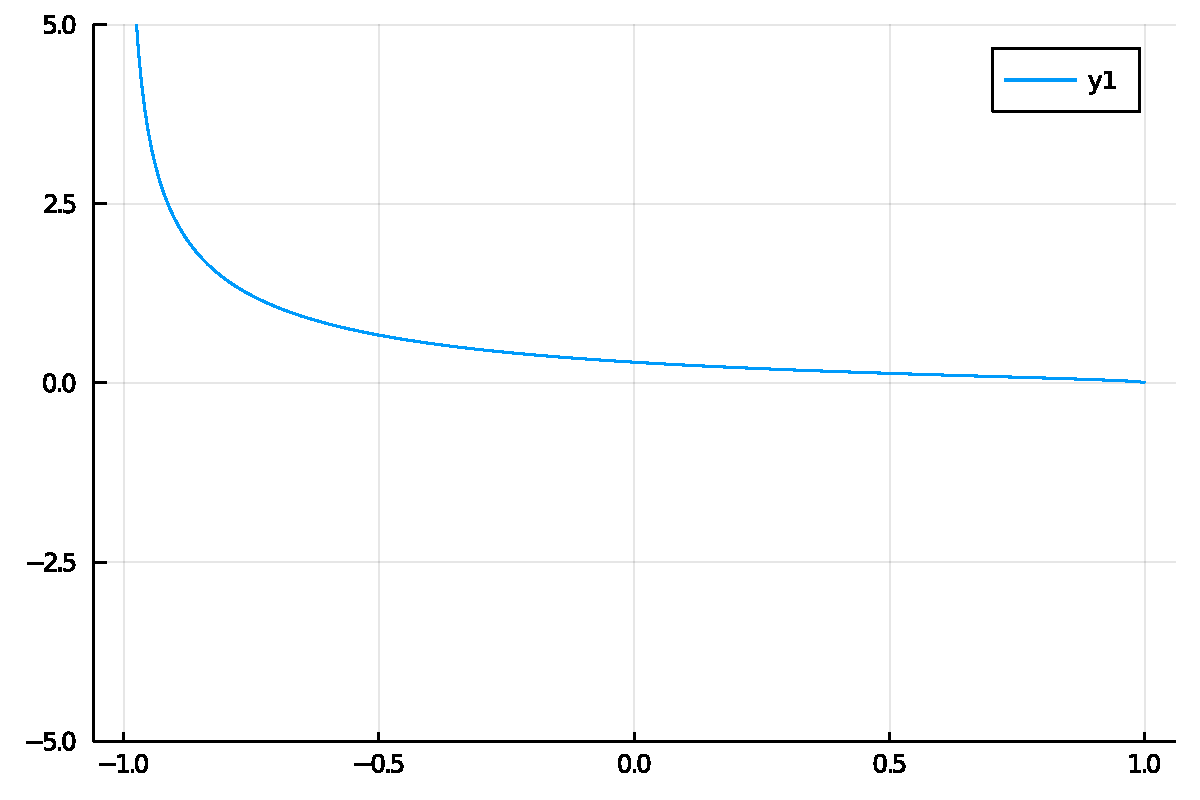
\includegraphics[width=\linewidth]{C:/Users/mfaso/OneDrive/Documents/GitHub/M3M6AppliedComplexAnalysis/output/figures/Solutions3_17_1.pdf}

\begin{lstlisting}
(*@\HLJLn{x}@*) (*@\HLJLoB{=}@*) (*@\HLJLnfB{0.1}@*)
(*@\HLJLnf{H}@*)(*@\HLJLp{(}@*)(*@\HLJLn{u}@*)(*@\HLJLp{,}@*)(*@\HLJLn{x}@*)(*@\HLJLp{)}@*) (*@\HLJLp{,}@*) (*@\HLJLni{1}@*)(*@\HLJLoB{/}@*)(*@\HLJLp{(}@*)(*@\HLJLni{2}@*)(*@\HLJLoB{+}@*)(*@\HLJLn{x}@*)(*@\HLJLp{)}@*)
\end{lstlisting}

\begin{lstlisting}
(0.47619047619047533, 0.47619047619047616)
\end{lstlisting}


\subsection{Problem 2.1}
Doing the change of variables $\zeta = b s$ we have

\[
\log(ab) = \int_1^{ab} {\D \zeta \over \zeta} = \int_{1/b}^a {\D s \over s}
\]
if $\gamma$ does not surround the origin, we have

\[
0 = \oint_\gamma {\D s \over s} = \left[\int_1^{1/b} + \int_{1/b}^a + \int_a^1\right] {\D s \over s}
\]
which implies

\[
\log(ab) = \left[-\int_a^1 -\int_1^{1/b} \right] {\D s \over s} = \log a - \log {1 \over b} = \log a + \log b
\]
Here's a picture:


\begin{lstlisting}
(*@\HLJLn{a}@*) (*@\HLJLoB{=}@*) (*@\HLJLnfB{1.0}@*)(*@\HLJLoB{+}@*)(*@\HLJLnfB{2.0}@*)(*@\HLJLn{im}@*)
(*@\HLJLn{b}@*) (*@\HLJLoB{=}@*) (*@\HLJLoB{-}@*)(*@\HLJLnfB{1.0}@*)(*@\HLJLoB{-}@*)(*@\HLJLnfB{2.0}@*)(*@\HLJLn{im}@*)

(*@\HLJLnd{@show}@*) (*@\HLJLnf{log}@*)(*@\HLJLp{(}@*)(*@\HLJLn{a}@*)(*@\HLJLoB{*}@*)(*@\HLJLn{b}@*)(*@\HLJLp{)}@*)
(*@\HLJLnd{@show}@*) (*@\HLJLnf{log}@*)(*@\HLJLp{(}@*)(*@\HLJLn{a}@*)(*@\HLJLp{)}@*) (*@\HLJLoB{+}@*) (*@\HLJLnf{log}@*)(*@\HLJLp{(}@*)(*@\HLJLn{b}@*)(*@\HLJLp{)}@*)

(*@\HLJLnf{scatter}@*)(*@\HLJLp{([}@*)(*@\HLJLnf{real}@*)(*@\HLJLp{(}@*)(*@\HLJLni{1}@*)(*@\HLJLoB{/}@*)(*@\HLJLn{b}@*)(*@\HLJLp{)],}@*) (*@\HLJLp{[}@*)(*@\HLJLnf{imag}@*)(*@\HLJLp{(}@*)(*@\HLJLni{1}@*)(*@\HLJLoB{/}@*)(*@\HLJLn{b}@*)(*@\HLJLp{)];}@*) (*@\HLJLn{label}@*)(*@\HLJLoB{=}@*)(*@\HLJLs{"{}1/b"{}}@*)(*@\HLJLp{)}@*)
(*@\HLJLnf{scatter!}@*)(*@\HLJLp{([}@*)(*@\HLJLnf{real}@*)(*@\HLJLp{(}@*)(*@\HLJLn{a}@*)(*@\HLJLp{)],}@*) (*@\HLJLp{[}@*)(*@\HLJLnf{imag}@*)(*@\HLJLp{(}@*)(*@\HLJLn{a}@*)(*@\HLJLp{)];}@*) (*@\HLJLn{label}@*)(*@\HLJLoB{=}@*)(*@\HLJLs{"{}a"{}}@*)(*@\HLJLp{)}@*)
(*@\HLJLnf{scatter!}@*)(*@\HLJLp{([}@*)(*@\HLJLnfB{0.0}@*)(*@\HLJLp{],}@*) (*@\HLJLp{[}@*)(*@\HLJLnfB{0.0}@*)(*@\HLJLp{];}@*) (*@\HLJLn{label}@*)(*@\HLJLoB{=}@*)(*@\HLJLs{"{}0"{}}@*)(*@\HLJLp{)}@*)
(*@\HLJLnf{plot!}@*)(*@\HLJLp{(}@*)(*@\HLJLnf{Segment}@*)(*@\HLJLp{(}@*)(*@\HLJLni{1}@*)(*@\HLJLp{,}@*) (*@\HLJLni{1}@*)(*@\HLJLoB{/}@*)(*@\HLJLn{b}@*)(*@\HLJLp{)}@*) (*@\HLJLoB{\ensuremath{\cup}}@*) (*@\HLJLnf{Segment}@*)(*@\HLJLp{(}@*)(*@\HLJLni{1}@*)(*@\HLJLoB{/}@*)(*@\HLJLn{b}@*)(*@\HLJLp{,}@*) (*@\HLJLn{a}@*)(*@\HLJLp{)}@*) (*@\HLJLoB{\ensuremath{\cup}}@*) (*@\HLJLnf{Segment}@*)(*@\HLJLp{(}@*)(*@\HLJLn{a}@*)(*@\HLJLp{,}@*) (*@\HLJLni{1}@*)(*@\HLJLp{);}@*) (*@\HLJLn{label}@*)(*@\HLJLoB{=}@*)(*@\HLJLs{"{}contour"{}}@*)(*@\HLJLp{)}@*)
\end{lstlisting}

\begin{lstlisting}
log(a * b) = 1.6094379124341003 - 0.9272952180016122im
log(a) + log(b) = 1.6094379124341003 - 0.9272952180016123im
\end{lstlisting}

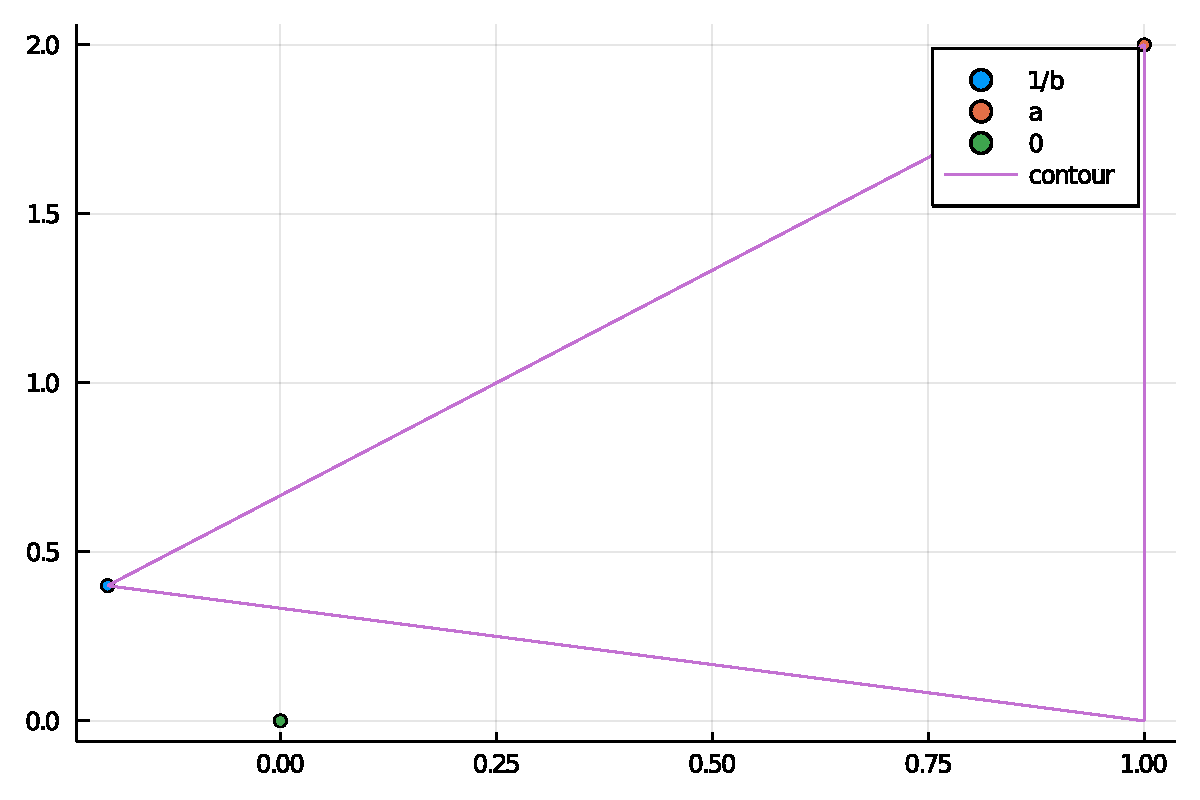
\includegraphics[width=\linewidth]{C:/Users/mfaso/OneDrive/Documents/GitHub/M3M6AppliedComplexAnalysis/output/figures/Solutions3_19_1.pdf}

If it surrounds the origin counbter-clockwise, that is, it has positive orientation, we have $2\pi \I = \oint_\gamma {\D s \over s}$, which shoes that

\[
\log(ab) = 2 \pi \I - \left[\int_a^1 +\int_1^{1/b} \right] {\D s \over s} = \log a + \log b + 2\pi \I
\]
and a similar result when counter clockwise.


\begin{lstlisting}
(*@\HLJLn{a}@*) (*@\HLJLoB{=}@*) (*@\HLJLnfB{1.0}@*)(*@\HLJLoB{+}@*)(*@\HLJLnfB{2.0}@*)(*@\HLJLn{im}@*)
(*@\HLJLn{b}@*) (*@\HLJLoB{=}@*) (*@\HLJLoB{-}@*)(*@\HLJLnfB{2.0}@*)(*@\HLJLoB{+}@*)(*@\HLJLnfB{2.0}@*)(*@\HLJLn{im}@*)

(*@\HLJLnd{@show}@*) (*@\HLJLnf{log}@*)(*@\HLJLp{(}@*)(*@\HLJLn{a}@*)(*@\HLJLoB{*}@*)(*@\HLJLn{b}@*)(*@\HLJLp{)}@*)
(*@\HLJLnd{@show}@*) (*@\HLJLnf{log}@*)(*@\HLJLp{(}@*)(*@\HLJLn{a}@*)(*@\HLJLp{)}@*) (*@\HLJLoB{+}@*) (*@\HLJLnf{log}@*)(*@\HLJLp{(}@*)(*@\HLJLn{b}@*)(*@\HLJLp{)}@*) (*@\HLJLoB{-}@*) (*@\HLJLni{2}@*)(*@\HLJLn{\ensuremath{\pi}}@*)(*@\HLJLoB{*}@*)(*@\HLJLn{im}@*)
(*@\HLJLnf{scatter}@*)(*@\HLJLp{([}@*)(*@\HLJLnf{real}@*)(*@\HLJLp{(}@*)(*@\HLJLni{1}@*)(*@\HLJLoB{/}@*)(*@\HLJLn{b}@*)(*@\HLJLp{)],}@*) (*@\HLJLp{[}@*)(*@\HLJLnf{imag}@*)(*@\HLJLp{(}@*)(*@\HLJLni{1}@*)(*@\HLJLoB{/}@*)(*@\HLJLn{b}@*)(*@\HLJLp{)];}@*) (*@\HLJLn{label}@*)(*@\HLJLoB{=}@*)(*@\HLJLs{"{}1/b"{}}@*)(*@\HLJLp{)}@*)
(*@\HLJLnf{scatter!}@*)(*@\HLJLp{([}@*)(*@\HLJLnf{real}@*)(*@\HLJLp{(}@*)(*@\HLJLn{a}@*)(*@\HLJLp{)],}@*) (*@\HLJLp{[}@*)(*@\HLJLnf{imag}@*)(*@\HLJLp{(}@*)(*@\HLJLn{a}@*)(*@\HLJLp{)];}@*) (*@\HLJLn{label}@*)(*@\HLJLoB{=}@*)(*@\HLJLs{"{}a"{}}@*)(*@\HLJLp{)}@*)
(*@\HLJLnf{scatter!}@*)(*@\HLJLp{([}@*)(*@\HLJLnfB{0.0}@*)(*@\HLJLp{],}@*) (*@\HLJLp{[}@*)(*@\HLJLnfB{0.0}@*)(*@\HLJLp{];}@*) (*@\HLJLn{label}@*)(*@\HLJLoB{=}@*)(*@\HLJLs{"{}0"{}}@*)(*@\HLJLp{)}@*)
(*@\HLJLnf{plot!}@*)(*@\HLJLp{(}@*)(*@\HLJLnf{Segment}@*)(*@\HLJLp{(}@*)(*@\HLJLni{1}@*)(*@\HLJLp{,}@*) (*@\HLJLni{1}@*)(*@\HLJLoB{/}@*)(*@\HLJLn{b}@*)(*@\HLJLp{)}@*) (*@\HLJLoB{\ensuremath{\cup}}@*) (*@\HLJLnf{Segment}@*)(*@\HLJLp{(}@*)(*@\HLJLni{1}@*)(*@\HLJLoB{/}@*)(*@\HLJLn{b}@*)(*@\HLJLp{,}@*) (*@\HLJLn{a}@*)(*@\HLJLp{)}@*) (*@\HLJLoB{\ensuremath{\cup}}@*) (*@\HLJLnf{Segment}@*)(*@\HLJLp{(}@*)(*@\HLJLn{a}@*)(*@\HLJLp{,}@*) (*@\HLJLni{1}@*)(*@\HLJLp{);}@*) (*@\HLJLn{label}@*)(*@\HLJLoB{=}@*)(*@\HLJLs{"{}contour"{}}@*)(*@\HLJLp{)}@*)
\end{lstlisting}

\begin{lstlisting}
log(a * b) = 1.8444397270569681 - 2.819842099193151im
(log(a) + log(b)) - (2(*@\ensuremath{\pi}@*() * im = 1.844439727056968 - 2.819842099193151im
\end{lstlisting}

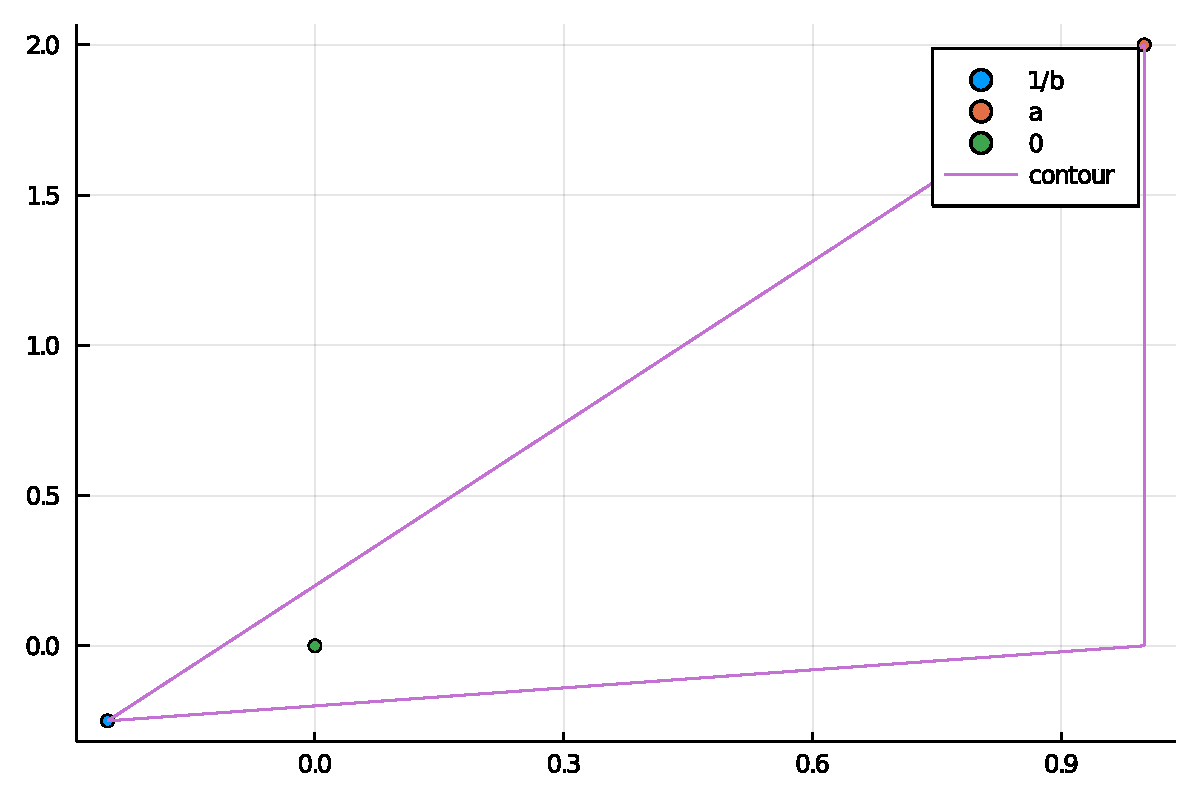
\includegraphics[width=\linewidth]{C:/Users/mfaso/OneDrive/Documents/GitHub/M3M6AppliedComplexAnalysis/output/figures/Solutions3_20_1.pdf}

If the contour passes through the origin, there are three possibility:

\begin{itemize}
\item[1. ] $[a,1]$ contains zero, hence $a < 0$


\item[2. ] \[
[1,1/b]
\]
contains zero, hence $b < 0$


\item[3. ] \[
[1/b, a]
\]
contains zero, which can only be true if $a b < 0$ by considering the equation of the line segment.

\end{itemize}
1. In the case where $a < 0$ and $b < 0$ (and hence $a b > 0$), perturbing $a$ above  and $b$ below or vice versa avoids $\gamma$ winding around zero, so we have

\[
\log(a b) = \log_+ a + \log_- b = \log_- a + \log_+ b = \log_+ a + \log_+ b - 2 \pi \I = \log_- a + \log_- b + 2 \pi \I
\]

\begin{lstlisting}
(*@\HLJLn{a}@*) (*@\HLJLoB{=}@*) (*@\HLJLoB{-}@*)(*@\HLJLnfB{2.0}@*)
(*@\HLJLn{b}@*) (*@\HLJLoB{=}@*) (*@\HLJLoB{-}@*)(*@\HLJLnfB{3.0}@*)

(*@\HLJLnd{@show}@*) (*@\HLJLnf{log}@*)(*@\HLJLp{(}@*)(*@\HLJLn{a}@*)(*@\HLJLoB{*}@*)(*@\HLJLn{b}@*)(*@\HLJLp{)}@*)
(*@\HLJLnd{@show}@*) (*@\HLJLnf{log}@*)(*@\HLJLp{(}@*)(*@\HLJLn{a}@*)(*@\HLJLoB{+}@*)(*@\HLJLnfB{0.0}@*)(*@\HLJLn{im}@*)(*@\HLJLp{)}@*) (*@\HLJLoB{+}@*) (*@\HLJLnf{log}@*)(*@\HLJLp{(}@*)(*@\HLJLn{b}@*)(*@\HLJLoB{-}@*)(*@\HLJLnfB{0.0}@*)(*@\HLJLn{im}@*)(*@\HLJLp{)}@*)
(*@\HLJLnd{@show}@*) (*@\HLJLnf{log}@*)(*@\HLJLp{(}@*)(*@\HLJLn{a}@*)(*@\HLJLoB{-}@*)(*@\HLJLnfB{0.0}@*)(*@\HLJLn{im}@*)(*@\HLJLp{)}@*) (*@\HLJLoB{+}@*) (*@\HLJLnf{log}@*)(*@\HLJLp{(}@*)(*@\HLJLn{b}@*)(*@\HLJLoB{+}@*)(*@\HLJLnfB{0.0}@*)(*@\HLJLn{im}@*)(*@\HLJLp{)}@*)
(*@\HLJLnd{@show}@*) (*@\HLJLnf{log}@*)(*@\HLJLp{(}@*)(*@\HLJLn{a}@*)(*@\HLJLoB{-}@*)(*@\HLJLnfB{0.0}@*)(*@\HLJLn{im}@*)(*@\HLJLp{)}@*) (*@\HLJLoB{+}@*) (*@\HLJLnf{log}@*)(*@\HLJLp{(}@*)(*@\HLJLn{b}@*)(*@\HLJLoB{-}@*)(*@\HLJLnfB{0.0}@*)(*@\HLJLn{im}@*)(*@\HLJLp{)}@*) (*@\HLJLoB{+}@*) (*@\HLJLni{2}@*)(*@\HLJLn{\ensuremath{\pi}}@*)(*@\HLJLoB{*}@*)(*@\HLJLn{im}@*)
(*@\HLJLnd{@show}@*) (*@\HLJLnf{log}@*)(*@\HLJLp{(}@*)(*@\HLJLn{a}@*)(*@\HLJLoB{+}@*)(*@\HLJLnfB{0.0}@*)(*@\HLJLn{im}@*)(*@\HLJLp{)}@*) (*@\HLJLoB{+}@*) (*@\HLJLnf{log}@*)(*@\HLJLp{(}@*)(*@\HLJLn{b}@*)(*@\HLJLoB{+}@*)(*@\HLJLnfB{0.0}@*)(*@\HLJLn{im}@*)(*@\HLJLp{)}@*) (*@\HLJLoB{-}@*) (*@\HLJLni{2}@*)(*@\HLJLn{\ensuremath{\pi}}@*)(*@\HLJLoB{*}@*)(*@\HLJLn{im}@*)(*@\HLJLp{;}@*)
\end{lstlisting}

\begin{lstlisting}
log(a * b) = 1.791759469228055
log(a + 0.0im) + log(b - 0.0im) = 1.791759469228055 + 0.0im
log(a - 0.0im) + log(b + 0.0im) = 1.791759469228055 + 0.0im
log(a - 0.0im) + log(b - 0.0im) + (2(*@\ensuremath{\pi}@*() * im = 1.791759469228055 + 0.0im
(log(a + 0.0im) + log(b + 0.0im)) - (2(*@\ensuremath{\pi}@*() * im = 1.791759469228055 + 0.0im
\end{lstlisting}


In the case where $a < 0$ and $b > 0$, then $a b < 0$, but we can perturb $a$ above/below to get

\[
\log_\pm(a b) = \log_\pm a + \log b
\]
(and by symmetry, the equivalent holds for $b < 0$ and $a > 0$.)


\begin{lstlisting}
(*@\HLJLn{a}@*) (*@\HLJLoB{=}@*) (*@\HLJLoB{-}@*)(*@\HLJLnfB{2.0}@*)
(*@\HLJLn{b}@*) (*@\HLJLoB{=}@*) (*@\HLJLnfB{3.0}@*)

(*@\HLJLnd{@show}@*) (*@\HLJLnf{log}@*)(*@\HLJLp{(}@*)(*@\HLJLn{a}@*)(*@\HLJLoB{*}@*)(*@\HLJLn{b}@*) (*@\HLJLoB{+}@*)(*@\HLJLnfB{0.0}@*)(*@\HLJLn{im}@*)(*@\HLJLp{)}@*)
(*@\HLJLnd{@show}@*) (*@\HLJLnf{log}@*)(*@\HLJLp{(}@*)(*@\HLJLn{a}@*)(*@\HLJLoB{+}@*)(*@\HLJLnfB{0.0}@*)(*@\HLJLn{im}@*)(*@\HLJLp{)}@*) (*@\HLJLoB{+}@*) (*@\HLJLnf{log}@*)(*@\HLJLp{(}@*)(*@\HLJLn{b}@*)(*@\HLJLp{);}@*)

(*@\HLJLnd{@show}@*) (*@\HLJLnf{log}@*)(*@\HLJLp{(}@*)(*@\HLJLn{a}@*)(*@\HLJLoB{*}@*)(*@\HLJLn{b}@*) (*@\HLJLoB{-}@*)(*@\HLJLnfB{0.0}@*)(*@\HLJLn{im}@*)(*@\HLJLp{)}@*)
(*@\HLJLnd{@show}@*) (*@\HLJLnf{log}@*)(*@\HLJLp{(}@*)(*@\HLJLn{a}@*)(*@\HLJLoB{-}@*)(*@\HLJLnfB{0.0}@*)(*@\HLJLn{im}@*)(*@\HLJLp{)}@*) (*@\HLJLoB{+}@*) (*@\HLJLnf{log}@*)(*@\HLJLp{(}@*)(*@\HLJLn{b}@*)(*@\HLJLp{);}@*)
\end{lstlisting}

\begin{lstlisting}
log(a * b + 0.0im) = 1.791759469228055 + 3.141592653589793im
log(a + 0.0im) + log(b) = 1.791759469228055 + 3.141592653589793im
log(a * b - 0.0im) = 1.791759469228055 - 3.141592653589793im
log(a - 0.0im) + log(b) = 1.791759469228055 - 3.141592653589793im
\end{lstlisting}


In the case where $a < 0$, if $\Im b > 0$ we can perturb $a$ below so that $\gamma$ does not contain zero, giving us

\[
\log(ab) = \log_- a + \log b
\]
similarly, if $\Im b < 0$ we can perturb $a$ above.


\begin{lstlisting}
(*@\HLJLn{a}@*) (*@\HLJLoB{=}@*) (*@\HLJLoB{-}@*)(*@\HLJLnfB{2.0}@*)
(*@\HLJLn{b}@*) (*@\HLJLoB{=}@*) (*@\HLJLnfB{3.0}@*) (*@\HLJLoB{+}@*) (*@\HLJLn{im}@*)

(*@\HLJLnd{@show}@*) (*@\HLJLnf{log}@*)(*@\HLJLp{(}@*)(*@\HLJLn{a}@*)(*@\HLJLoB{*}@*)(*@\HLJLn{b}@*)(*@\HLJLp{)}@*)
(*@\HLJLnd{@show}@*) (*@\HLJLnf{log}@*)(*@\HLJLp{(}@*)(*@\HLJLn{a}@*)(*@\HLJLoB{-}@*)(*@\HLJLnfB{0.0}@*)(*@\HLJLn{im}@*)(*@\HLJLp{)}@*) (*@\HLJLoB{+}@*) (*@\HLJLnf{log}@*)(*@\HLJLp{(}@*)(*@\HLJLn{b}@*)(*@\HLJLp{);}@*)

(*@\HLJLn{b}@*) (*@\HLJLoB{=}@*) (*@\HLJLnfB{3.0}@*) (*@\HLJLoB{+}@*) (*@\HLJLn{im}@*)(*@\HLJLp{;}@*)
(*@\HLJLnd{@show}@*) (*@\HLJLnf{log}@*)(*@\HLJLp{(}@*)(*@\HLJLn{a}@*)(*@\HLJLoB{*}@*)(*@\HLJLn{b}@*)(*@\HLJLp{)}@*)
(*@\HLJLnd{@show}@*) (*@\HLJLnf{log}@*)(*@\HLJLp{(}@*)(*@\HLJLn{a}@*)(*@\HLJLoB{+}@*)(*@\HLJLnfB{0.0}@*)(*@\HLJLn{im}@*)(*@\HLJLp{)}@*) (*@\HLJLoB{+}@*) (*@\HLJLnf{log}@*)(*@\HLJLp{(}@*)(*@\HLJLn{b}@*)(*@\HLJLp{);}@*)
\end{lstlisting}

\begin{lstlisting}
log(a * b) = 1.8444397270569681 - 2.819842099193151im
log(a - 0.0im) + log(b) = 1.8444397270569683 - 2.819842099193151im
log(a * b) = 1.8444397270569681 - 2.819842099193151im
log(a + 0.0im) + log(b) = 1.8444397270569683 + 3.4633432079864352im
\end{lstlisting}


2. In this case, swap the role of $a$ and $b$ and use the answers for $a < 0$.

3. Finally, we have the case $a b < 0$ and neither $a$ nor $b$ is real. Note that

\[
ab = (a_x + \I a_y) (b_x + \I b_y) = a_x b_x - a_y b_y +  \I(a_x b_y + a_yb_x)
\]
It follows if $b_x > 0$ we have

\[
(ab)_+ = a_+ b
\]
and if $b_x < 0$ we have

\[
(ab)_+ = a_- b
\]

\begin{lstlisting}
(*@\HLJLn{a}@*) (*@\HLJLoB{=}@*) (*@\HLJLoB{-}@*)(*@\HLJLnfB{1.0}@*) (*@\HLJLoB{+}@*) (*@\HLJLnfB{1.0}@*)(*@\HLJLn{im}@*)
(*@\HLJLn{b}@*) (*@\HLJLoB{=}@*) (*@\HLJLnfB{1.0}@*) (*@\HLJLoB{+}@*) (*@\HLJLnfB{1.0}@*)(*@\HLJLn{im}@*)
(*@\HLJLnd{@show}@*) (*@\HLJLnf{log}@*)(*@\HLJLp{(}@*)(*@\HLJLn{a}@*)(*@\HLJLoB{*}@*)(*@\HLJLn{b}@*) (*@\HLJLoB{+}@*)  (*@\HLJLnf{eps}@*)(*@\HLJLp{()}@*)(*@\HLJLn{im}@*)(*@\HLJLp{)}@*)
(*@\HLJLnd{@show}@*) (*@\HLJLnf{log}@*)(*@\HLJLp{((}@*)(*@\HLJLn{a}@*)(*@\HLJLoB{+}@*)(*@\HLJLnf{eps}@*)(*@\HLJLp{()}@*)(*@\HLJLn{im}@*)(*@\HLJLp{)}@*)(*@\HLJLoB{*}@*)(*@\HLJLn{b}@*)(*@\HLJLp{)}@*)

(*@\HLJLn{a}@*) (*@\HLJLoB{=}@*) (*@\HLJLnfB{1.0}@*) (*@\HLJLoB{+}@*) (*@\HLJLnfB{1.0}@*)(*@\HLJLn{im}@*)
(*@\HLJLn{b}@*) (*@\HLJLoB{=}@*) (*@\HLJLoB{-}@*)(*@\HLJLnfB{1.0}@*) (*@\HLJLoB{+}@*) (*@\HLJLnfB{1.0}@*)(*@\HLJLn{im}@*)
(*@\HLJLnd{@show}@*) (*@\HLJLnf{log}@*)(*@\HLJLp{(}@*)(*@\HLJLn{a}@*)(*@\HLJLoB{*}@*)(*@\HLJLn{b}@*) (*@\HLJLoB{+}@*)  (*@\HLJLnf{eps}@*)(*@\HLJLp{()}@*)(*@\HLJLn{im}@*)(*@\HLJLp{)}@*)
(*@\HLJLnd{@show}@*) (*@\HLJLnf{log}@*)(*@\HLJLp{((}@*)(*@\HLJLn{a}@*)(*@\HLJLoB{-}@*)(*@\HLJLnf{eps}@*)(*@\HLJLp{()}@*)(*@\HLJLn{im}@*)(*@\HLJLp{)}@*)(*@\HLJLoB{*}@*)(*@\HLJLn{b}@*)(*@\HLJLp{)}@*)
\end{lstlisting}

\begin{lstlisting}
log(a * b + eps() * im) = 0.6931471805599453 + 3.141592653589793im
log((a + eps() * im) * b) = 0.6931471805599453 + 3.141592653589793im
log(a * b + eps() * im) = 0.6931471805599453 + 3.141592653589793im
log((a - eps() * im) * b) = 0.6931471805599452 + 3.141592653589793im
0.6931471805599452 + 3.141592653589793im
\end{lstlisting}


We can use this perturbation to reduce to the previous cases. For example, if $a = 1 + \I$ and $b = -1 + \I$, pertubing $ab$ above causes $a$ to be perturbed  above, which causes the contour to surround the origin clockwise, hence we have

\[
\log_+(ab) = \log(a)_+b = \log a b - 2 \pi \I
\]

\begin{lstlisting}
(*@\HLJLn{a}@*) (*@\HLJLoB{=}@*) (*@\HLJLnfB{1.0}@*) (*@\HLJLoB{+}@*) (*@\HLJLnfB{1.0}@*)(*@\HLJLn{im}@*)
(*@\HLJLn{b}@*) (*@\HLJLoB{=}@*) (*@\HLJLoB{-}@*)(*@\HLJLnfB{1.0}@*) (*@\HLJLoB{+}@*) (*@\HLJLnfB{1.0}@*)(*@\HLJLn{im}@*)
(*@\HLJLnd{@show}@*) (*@\HLJLnf{log}@*)(*@\HLJLp{(}@*)(*@\HLJLn{a}@*)(*@\HLJLoB{*}@*)(*@\HLJLn{b}@*) (*@\HLJLoB{-}@*)  (*@\HLJLnf{eps}@*)(*@\HLJLp{()}@*)(*@\HLJLn{im}@*)(*@\HLJLp{)}@*)
(*@\HLJLnd{@show}@*) (*@\HLJLnf{log}@*)(*@\HLJLp{(}@*)(*@\HLJLn{a}@*)(*@\HLJLp{)}@*)(*@\HLJLoB{+}@*)(*@\HLJLnf{log}@*)(*@\HLJLp{(}@*)(*@\HLJLn{b}@*)(*@\HLJLp{)}@*)(*@\HLJLoB{-}@*)(*@\HLJLni{2}@*)(*@\HLJLn{\ensuremath{\pi}}@*)(*@\HLJLoB{*}@*)(*@\HLJLn{im}@*)(*@\HLJLp{;}@*)
\end{lstlisting}

\begin{lstlisting}
log(a * b - eps() * im) = 0.6931471805599453 - 3.141592653589793im
(log(a) + log(b)) - (2(*@\ensuremath{\pi}@*() * im = 0.6931471805599453 - 3.141592653589793im
\end{lstlisting}


\subsection{Problem 2.2}
Use the contour $\gamma(t) = 1 + t(z-1)$ to reduce it to a normal integral: $\overline{\log z } = \overline{\int_1^z {1 \over \zeta} \D \zeta} = \overline{\int_0^1 {(z-1) \over 1+(z-1) t} \dt}  = \int_0^1 {(\bar z-1) \over 1+(\bar z-1) t} \dt = \int_1^{\bar z} {\D \zeta \over \zeta} = \log \bar z.$ We then have, since the contour from $1$ to $1/(\bar z)$ to $z$ never surrounds the origin since both $\Im z$ and $\Im 1/(\bar z)$ have the same sign, we have

\[
2 \Re \log z = \log z + \overline{\log z} = \log z + \log \bar z = \log z \bar z = \log |z|^2 = 2 \log |z|
\]
On the other hand, we have, where the contour of integration is chosen to be to the right of zero and then we do the change of variables $\zeta = |z| \E^{\I \theta}$

\[
2 \Im \log z = \log z - \log \bar z = \int_{\bar z}^z {\D \zeta \over \zeta} = \I \int_{-\arg z}^{\arg z} \D \theta = 2 \I \arg z
\]
\subsection{Problem 2.3}
We first show that it is analytic on $(-\infty,0)$. To do this, we need to show that the limit from above equals the limit from below: for $x < 0$ we have $\log_1^+ x -\log_1^- x = \log_+x - \log_- x -2 \pi \I = 0$ Then for $x > 0$ and using $\log_1^\pm(x) = \lim_{\epsilon\rightarrow 0} \log(x\pm \I \epsilon)$ we find

\[
\log_1^+(x) - \log_1^-x = \log x- \log x- 2\pi \I = -2 \pi \I
\]
\emph{Demonstration} Here we see that the following is the analytic continuation:


\begin{lstlisting}
(*@\HLJLn{log1}@*) (*@\HLJLoB{=}@*) (*@\HLJLn{z}@*) (*@\HLJLoB{->}@*) (*@\HLJLk{begin}@*)
    (*@\HLJLk{if}@*) (*@\HLJLnf{imag}@*)(*@\HLJLp{(}@*)(*@\HLJLn{z}@*)(*@\HLJLp{)}@*) (*@\HLJLoB{>}@*) (*@\HLJLni{0}@*)
        (*@\HLJLnf{log}@*)(*@\HLJLp{(}@*)(*@\HLJLn{z}@*)(*@\HLJLp{)}@*)
    (*@\HLJLk{elseif}@*) (*@\HLJLnf{imag}@*)(*@\HLJLp{(}@*)(*@\HLJLn{z}@*)(*@\HLJLp{)}@*) (*@\HLJLoB{==}@*) (*@\HLJLni{0}@*) (*@\HLJLoB{{\&}{\&}}@*) (*@\HLJLnf{real}@*)(*@\HLJLp{(}@*)(*@\HLJLn{z}@*)(*@\HLJLp{)}@*) (*@\HLJLoB{<}@*) (*@\HLJLni{0}@*)
        (*@\HLJLnf{log}@*)(*@\HLJLp{(}@*)(*@\HLJLn{z}@*) (*@\HLJLoB{+}@*) (*@\HLJLnfB{0.0}@*)(*@\HLJLn{im}@*)(*@\HLJLp{)}@*)
    (*@\HLJLk{elseif}@*) (*@\HLJLnf{imag}@*)(*@\HLJLp{(}@*)(*@\HLJLn{z}@*)(*@\HLJLp{)}@*) (*@\HLJLoB{<}@*) (*@\HLJLni{0}@*)
        (*@\HLJLnf{log}@*)(*@\HLJLp{(}@*)(*@\HLJLn{z}@*)(*@\HLJLp{)}@*) (*@\HLJLoB{+}@*) (*@\HLJLni{2}@*)(*@\HLJLn{\ensuremath{\pi}}@*)(*@\HLJLoB{*}@*)(*@\HLJLn{im}@*)
    (*@\HLJLk{else}@*)
            (*@\HLJLnf{error}@*)(*@\HLJLp{(}@*)(*@\HLJLs{"{}log1}@*) (*@\HLJLs{not}@*) (*@\HLJLs{defined}@*) (*@\HLJLs{on}@*) (*@\HLJLs{real}@*) (*@\HLJLs{axis"{}}@*)(*@\HLJLp{)}@*)
    (*@\HLJLk{end}@*)
(*@\HLJLk{end}@*)

(*@\HLJLnf{phaseplot}@*)(*@\HLJLp{(}@*)(*@\HLJLoB{-}@*)(*@\HLJLnfB{3..3}@*)(*@\HLJLp{,}@*) (*@\HLJLoB{-}@*)(*@\HLJLnfB{3..3}@*)(*@\HLJLp{,}@*) (*@\HLJLn{log1}@*)(*@\HLJLp{)}@*)
\end{lstlisting}

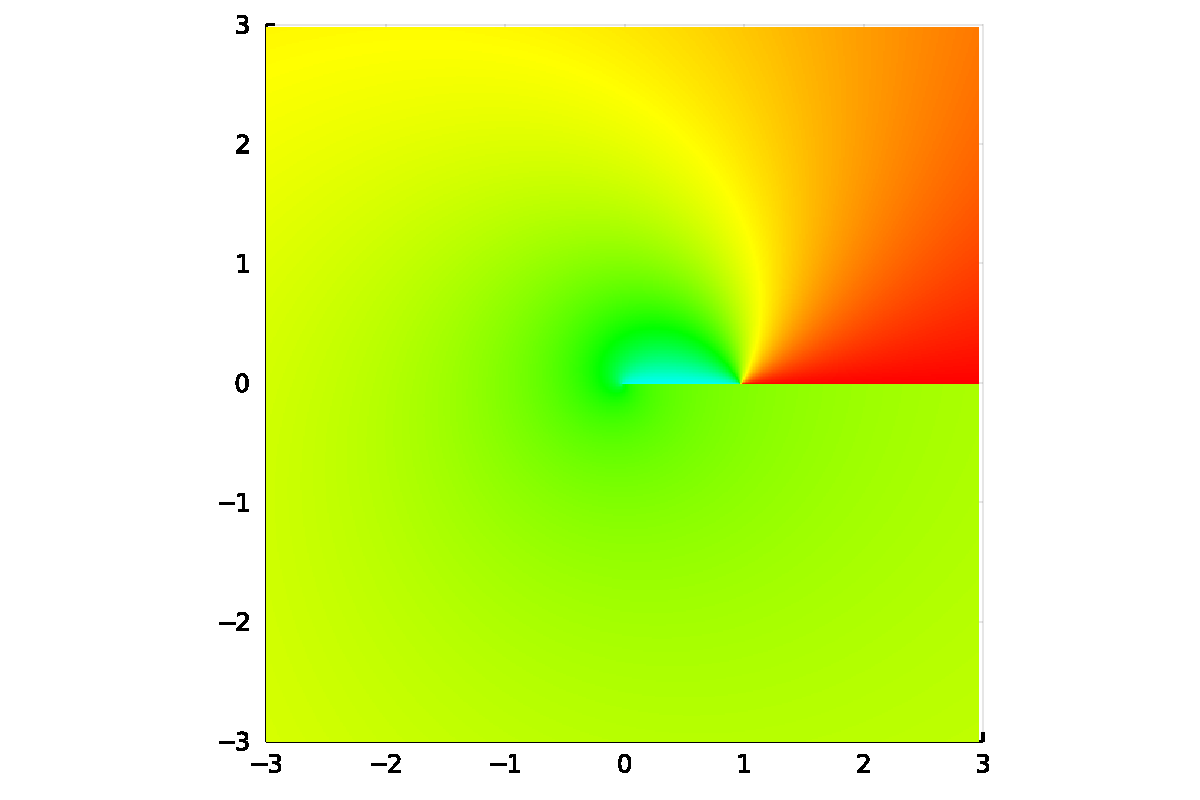
\includegraphics[width=\linewidth]{C:/Users/mfaso/OneDrive/Documents/GitHub/M3M6AppliedComplexAnalysis/output/figures/Solutions3_26_1.pdf}

\subsection{Problem 3.1}
\begin{itemize}
\item[1. ] Because it's absolutely integrable, we can exchange derivatives and integrals to determine

\end{itemize}
\[
{\D \CC f \over \D z} = {1 \over 2 \pi \I} \oint {f(\zeta)\over (\zeta-z)^2} \D \zeta
\]
\begin{itemize}
\item[2. ] There are two different possible approaches:

\begin{itemize}
\item the subtract and add back in technique: since $f$ is analytic for $z$ near $\zeta$, we can write

\end{itemize}
\end{itemize}
\[
\CC f(z) = {1 \over 2 \pi \I} \oint {f(\zeta)-f(z) \over \zeta-z} \D \zeta + f(z) \CC 1(z)
\]
Therefore

\[
\CC^+ f(\zeta) - \CC^- f(\zeta) = f(\zeta)( \CC^+ 1(\zeta) - \CC^- 1(\zeta))
\]
But we know (using Cauchy's integral formula / Residue calculus)

\[
\CC 1(z) = \begin{cases} 1 & |z| < 1 \\
                            0 & |z| > 1
                            \end{cases}
\]
hence $(\CC^+-\CC^-)1(\zeta) = 1$

\begin{itemize}
\item Since $f$ is analytic, we have for any radius $R > 1$ but inside the annulus

\end{itemize}
\[
\CC^+ f(\zeta) = {1 \over 2 \pi \I} \oint_{|\zeta| = R} {f(\zeta) \over \zeta -z} \D\zeta
\]
Similarly, for $\CC^-f(\zeta)$ with any radius $r < 1$ but inside the annulus. Therfore,

\[
\CC^+ f(\zeta) - \CC^- f(\zeta) = {1 \over 2 \pi \I} \left[\oint_{|\zeta| = R} - \oint_{|\zeta| = r} \right] {f(\zeta) \over \zeta -z} \D\zeta
\]
Deforming the contour and using Cauchy-integral formula gives the result.

\begin{itemize}
\item[3. ] This follow since ${1 \over \zeta - z} \rightarrow 0$ uniformly.

\end{itemize}
\subsection{Problem 3.2}
Suppose we have another solution $\phi$ and consider $\psi(z) = \phi(z) - \CC f(z)$. Then on the circle we have

\[
\psi_+(\zeta) - \psi_-(\zeta) = \phi_+(\zeta) - \CC_+f(\zeta) - \phi_-(\zeta) + \CC_+f(\zeta) = f(\zeta)-f(\zeta) = 0
\]
Thus $\psi$ is entire, and since it decays at infinity, it must be zero by Liouville's theorem.

\subsection{Problem 3.3}
When $k \geq 0$, we have from 3.1 and 3.2

\[
\CC[\diamond^k](z) =\begin{cases}
    z^k  & |z| < 1 \\
    0 & |z| > 1
    \end{cases}
\]
when $k < 0$ since $\CC[\diamond^k]^+(\zeta) - \CC[\diamond^k]^-(\zeta) = \zeta^k - 0 = \zeta^k$. we similarly have

\[
\CC[\diamond^k](z) =\begin{cases}
0  & |z| < 1 \\
    -z^k & |z| > 1
        \end{cases}
\]
Therefore,

\[
\Im \CC^-[\diamond^k](\zeta) =\begin{cases}
0  & k \geq 0 \\
    -{\zeta^k - \zeta^{-k} \over 2 \I} & k < 0
        \end{cases}
\]
and

\[
\Re \CC^-[\diamond^k](\zeta) =\begin{cases}
0  & k \geq 0 \\
    -{\zeta^k + \zeta^{-k} \over 2} & k < 0
        \end{cases}
\]
\subsection{Problem 3.4}
Express the solution outside the circle as

\[
v(x,y) = \Im ( \E^{-\I \theta} z + \CC f(z))
\]
for a to-be-determined $f$. On the circle, this reduces to

\[
\Im \CC^- f(\zeta) = -\cos \theta {\zeta - \zeta^{-1} \over 2 \I}  + \sin \theta {\zeta + \zeta^{-1} \over 2}
\]
Unlike the real case, we can include imaginary coefficients, thus the solution is

\[
f(\zeta) = (\cos \theta + \I \sin \theta) \zeta^{-1}
\]
and thus the full solution is

\[
v(x,y) =  \Im ( \E^{-\I \theta} z - \E^{\I \theta}   z^{-1}))
\]

\begin{lstlisting}
(*@\HLJLn{\ensuremath{\theta}}@*) (*@\HLJLoB{=}@*) (*@\HLJLnfB{0.1}@*)
(*@\HLJLn{v}@*) (*@\HLJLoB{=}@*) (*@\HLJLp{(}@*)(*@\HLJLn{x}@*)(*@\HLJLp{,}@*)(*@\HLJLn{y}@*)(*@\HLJLp{)}@*) (*@\HLJLoB{->}@*) (*@\HLJLn{x}@*)(*@\HLJLoB{{\textasciicircum}}@*)(*@\HLJLni{2}@*) (*@\HLJLoB{+}@*) (*@\HLJLn{y}@*)(*@\HLJLoB{{\textasciicircum}}@*)(*@\HLJLni{2}@*) (*@\HLJLoB{<}@*) (*@\HLJLni{1}@*) (*@\HLJLoB{?}@*) (*@\HLJLni{0}@*) (*@\HLJLoB{:}@*) (*@\HLJLnf{imag}@*)(*@\HLJLp{(}@*)(*@\HLJLnf{exp}@*)(*@\HLJLp{(}@*)(*@\HLJLoB{-}@*)(*@\HLJLn{im}@*)(*@\HLJLoB{*}@*)(*@\HLJLn{\ensuremath{\theta}}@*)(*@\HLJLp{)}@*) (*@\HLJLoB{*}@*) (*@\HLJLp{(}@*)(*@\HLJLn{x}@*)(*@\HLJLoB{+}@*)(*@\HLJLn{im}@*)(*@\HLJLoB{*}@*)(*@\HLJLn{y}@*)(*@\HLJLp{)}@*) (*@\HLJLoB{+}@*) (*@\HLJLnf{exp}@*)(*@\HLJLp{(}@*)(*@\HLJLn{im}@*)(*@\HLJLoB{*}@*)(*@\HLJLn{\ensuremath{\theta}}@*)(*@\HLJLp{)}@*) (*@\HLJLoB{*}@*) (*@\HLJLp{(}@*)(*@\HLJLn{x}@*)(*@\HLJLoB{+}@*)(*@\HLJLn{im}@*)(*@\HLJLoB{*}@*)(*@\HLJLn{y}@*)(*@\HLJLp{)}@*)(*@\HLJLoB{{\textasciicircum}}@*)(*@\HLJLp{(}@*)(*@\HLJLoB{-}@*)(*@\HLJLni{1}@*)(*@\HLJLp{))}@*)

(*@\HLJLn{xx}@*) (*@\HLJLoB{=}@*) (*@\HLJLoB{-}@*)(*@\HLJLni{8}@*)(*@\HLJLoB{:}@*)(*@\HLJLnfB{0.01}@*)(*@\HLJLoB{:}@*)(*@\HLJLni{8}@*)(*@\HLJLp{;}@*) (*@\HLJLn{yy}@*) (*@\HLJLoB{=}@*) (*@\HLJLoB{-}@*)(*@\HLJLni{5}@*)(*@\HLJLoB{:}@*)(*@\HLJLnfB{0.01}@*)(*@\HLJLoB{:}@*)(*@\HLJLni{5}@*)

(*@\HLJLnf{contour}@*)(*@\HLJLp{(}@*)(*@\HLJLn{xx}@*)(*@\HLJLp{,}@*) (*@\HLJLn{yy}@*)(*@\HLJLp{,}@*) (*@\HLJLn{v}@*)(*@\HLJLoB{.}@*)(*@\HLJLp{(}@*)(*@\HLJLn{xx}@*)(*@\HLJLoB{{\textquotesingle}}@*)(*@\HLJLp{,}@*) (*@\HLJLn{yy}@*)(*@\HLJLp{);}@*) (*@\HLJLn{nlevels}@*)(*@\HLJLoB{=}@*)(*@\HLJLni{100}@*)(*@\HLJLp{,}@*) (*@\HLJLn{ratio}@*)(*@\HLJLoB{=}@*)(*@\HLJLnfB{1.0}@*)(*@\HLJLp{)}@*)
(*@\HLJLnf{plot!}@*)(*@\HLJLp{(}@*)(*@\HLJLnf{Circle}@*)(*@\HLJLp{();}@*) (*@\HLJLn{color}@*)(*@\HLJLoB{=:}@*)(*@\HLJLn{black}@*)(*@\HLJLp{,}@*) (*@\HLJLn{legend}@*)(*@\HLJLoB{=}@*)(*@\HLJLkc{false}@*)(*@\HLJLp{)}@*)
\end{lstlisting}

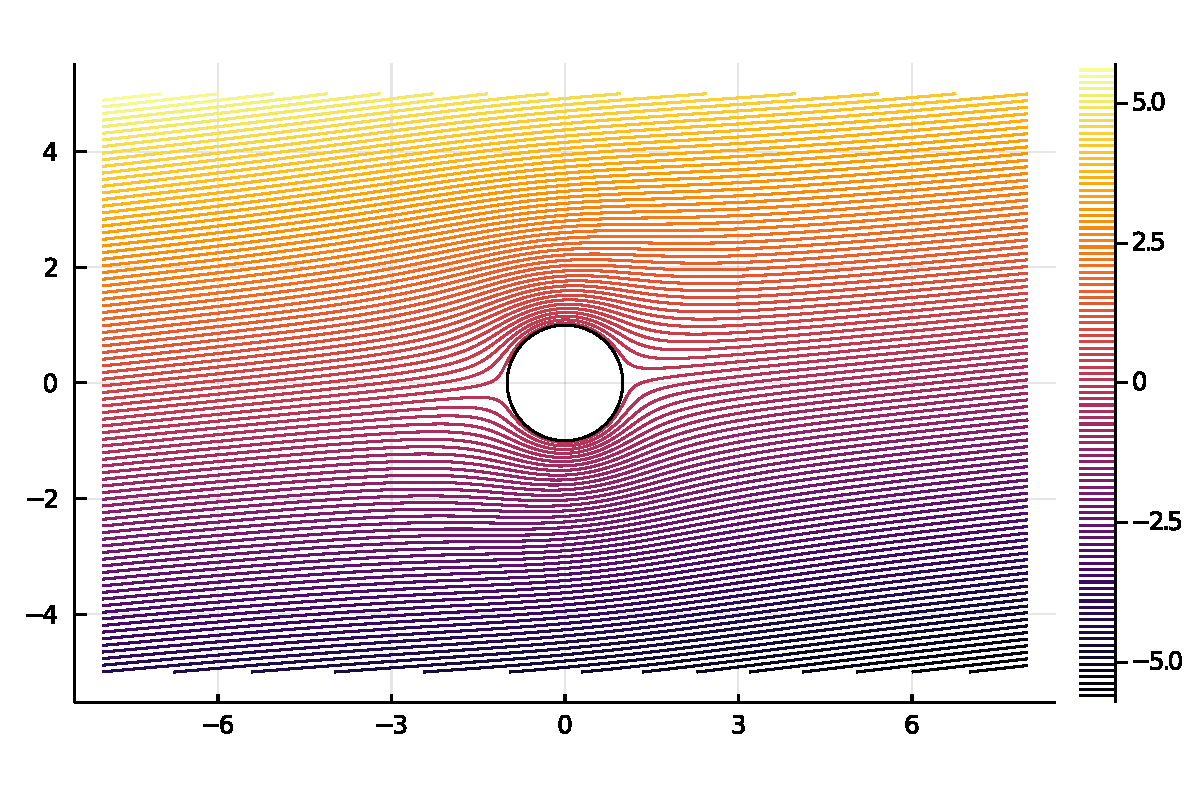
\includegraphics[width=\linewidth]{C:/Users/mfaso/OneDrive/Documents/GitHub/M3M6AppliedComplexAnalysis/output/figures/Solutions3_27_1.pdf}

\#\# Problem 4.1

\[
z^\alpha
\]
has the limits $z_\pm^\alpha = \E^{\pm \I  \pi \alpha} |z|^\alpha$, thus choose $\alpha = -{\theta \over 2\pi}$ where if we take $0 < \theta < 2\pi$ we have $0 < \alpha < 1$ (the case $\theta = 0$ and $\theta = \pi$ are covered by the Cauchy transform, that is ). Then consider

\[
\kappa(z) = (z-1)^{-\alpha} (z+1)^{\alpha-1}
\]
which has weaker than pole singularities and satisfies $\kappa(z) \sim z^{-1}$. For $-1 < x < 1$ it has the right jump

\begin{align*}
\kappa_+(x) &= (x-1)_+^{-\alpha} (x+1)^{\alpha - 1}  = \E^{-\I \pi \alpha} (1-x)^{-\alpha} (x+1)^{\alpha-1} = \E^{-2\I \pi \alpha} (x-1)_-^{-\alpha} (x+1)^{\alpha-1}\\
& = \E^{-2 \I \pi \alpha} \kappa_-(x)= \E^{\I \theta} \kappa_-(x)
\end{align*}
and  for $x < -1$ it has the jump

\[
\kappa_+(x) = (x-1)_+^{-\alpha} (x+1)_+^{\alpha-1}  = \E^{-\I \pi \alpha}\E^{\I \pi (\alpha-1)} (1-x)^{-\alpha} (-1-x)^{\alpha-1} =  \kappa_-(x)
\]
hence $\kappa$ is analytic.

We need to show this times a constant spans the entire space. Suppose we have another solution $\tilde \kappa$ and consider $r(z) = {\tilde \kappa(z) \over \kappa(z)}$. Note by construction that $\kappa$ has no zeros. Then

\[
r_+(x) = {\tilde\kappa_+(x) \over \kappa_+(x)} = {\tilde\kappa_-(x) \over \kappa_-(x)} = r_-(x)
\]
hence $r$ is analytic on $(-1,1)$. It has weaker than pole singularities because $\kappa(z)^{-1}$ is actually bounded at $\pm 1$. Therefore $r$ is bounded and entire, and thus must be a constant $r(z) \equiv r$, and thence $\tilde \kappa(z) = r \kappa(z)$.


\begin{lstlisting}
(*@\HLJLn{\ensuremath{\theta}}@*) (*@\HLJLoB{=}@*)(*@\HLJLnfB{2.3}@*)
(*@\HLJLn{\ensuremath{\alpha}}@*) (*@\HLJLoB{=}@*) (*@\HLJLoB{-}@*)(*@\HLJLn{\ensuremath{\theta}}@*)(*@\HLJLoB{/}@*)(*@\HLJLp{(}@*)(*@\HLJLni{2}@*)(*@\HLJLn{\ensuremath{\pi}}@*)(*@\HLJLp{)}@*)
(*@\HLJLn{\ensuremath{\kappa}}@*) (*@\HLJLoB{=}@*) (*@\HLJLn{z}@*) (*@\HLJLoB{->}@*) (*@\HLJLp{(}@*)(*@\HLJLn{z}@*)(*@\HLJLoB{-}@*)(*@\HLJLni{1}@*)(*@\HLJLp{)}@*)(*@\HLJLoB{{\textasciicircum}}@*)(*@\HLJLp{(}@*)(*@\HLJLoB{-}@*)(*@\HLJLn{\ensuremath{\alpha}}@*)(*@\HLJLp{)}@*)(*@\HLJLoB{*}@*)(*@\HLJLp{(}@*)(*@\HLJLn{z}@*)(*@\HLJLoB{+}@*)(*@\HLJLni{1}@*)(*@\HLJLp{)}@*)(*@\HLJLoB{{\textasciicircum}}@*)(*@\HLJLp{(}@*)(*@\HLJLn{\ensuremath{\alpha}}@*)(*@\HLJLoB{-}@*)(*@\HLJLni{1}@*)(*@\HLJLp{)}@*)
(*@\HLJLnf{\ensuremath{\kappa}}@*)(*@\HLJLp{(}@*)(*@\HLJLnfB{0.1}@*)(*@\HLJLoB{+}@*)(*@\HLJLnfB{0.0}@*)(*@\HLJLn{im}@*)(*@\HLJLp{)}@*) (*@\HLJLoB{-}@*) (*@\HLJLnf{exp}@*)(*@\HLJLp{(}@*)(*@\HLJLn{im}@*)(*@\HLJLoB{*}@*)(*@\HLJLn{\ensuremath{\theta}}@*)(*@\HLJLp{)}@*)(*@\HLJLoB{*}@*)(*@\HLJLnf{\ensuremath{\kappa}}@*)(*@\HLJLp{(}@*)(*@\HLJLnfB{0.1}@*)(*@\HLJLoB{-}@*)(*@\HLJLnfB{0.0}@*)(*@\HLJLn{im}@*)(*@\HLJLp{),}@*)(*@\HLJLnf{\ensuremath{\kappa}}@*)(*@\HLJLp{(}@*)(*@\HLJLnfB{100.0}@*)(*@\HLJLp{)}@*)
\end{lstlisting}

\begin{lstlisting}
(0.0 + 1.1102230246251565e-16im, 0.00982876598532333)
\end{lstlisting}


\begin{lstlisting}
(*@\HLJLnf{phaseplot}@*)(*@\HLJLp{(}@*)(*@\HLJLoB{-}@*)(*@\HLJLnfB{3..3}@*)(*@\HLJLp{,}@*) (*@\HLJLoB{-}@*)(*@\HLJLnfB{3..3}@*)(*@\HLJLp{,}@*) (*@\HLJLn{\ensuremath{\kappa}}@*)(*@\HLJLp{)}@*)
\end{lstlisting}

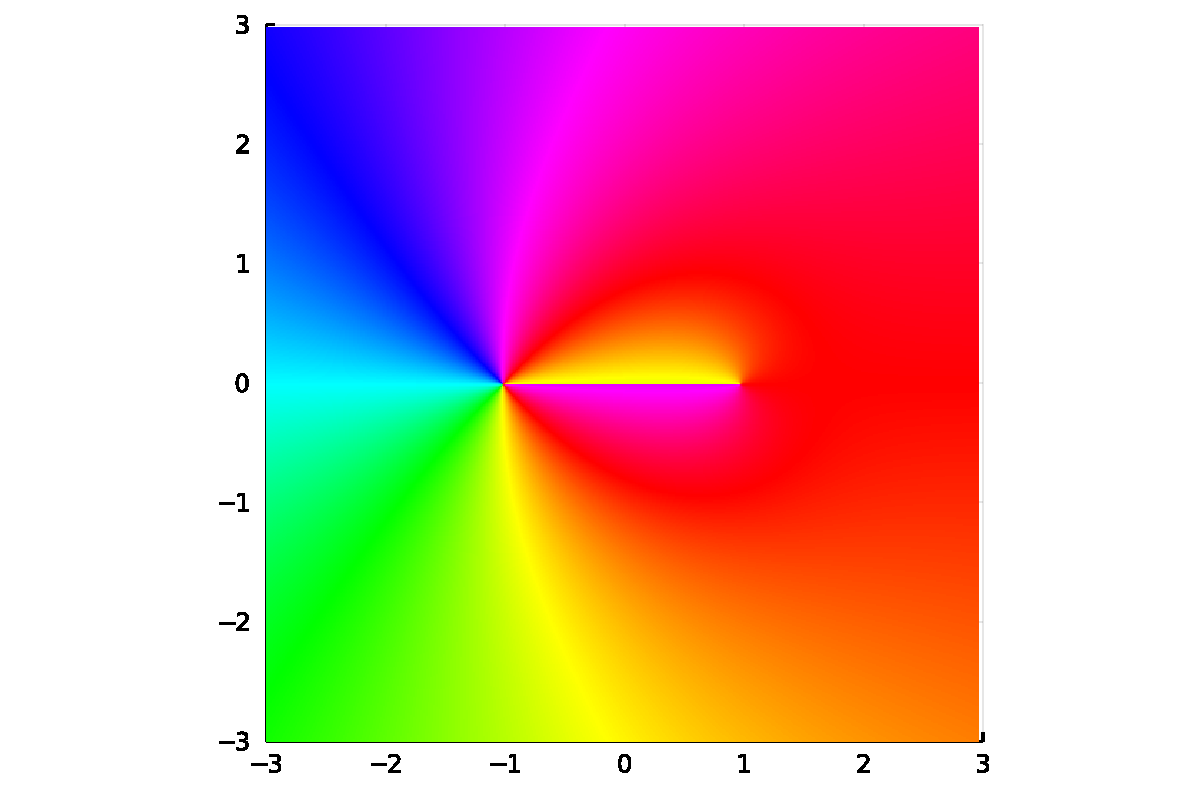
\includegraphics[width=\linewidth]{C:/Users/mfaso/OneDrive/Documents/GitHub/M3M6AppliedComplexAnalysis/output/figures/Solutions3_29_1.pdf}

\subsection{Problem 4.2}
We want to mimic the solution of $\phi_+(x) + \phi_-(x)$. So take

\[
\phi(z) = \kappa(z) \CC\br[{f \over \kappa_+}](z) =\E^{-\I \theta/2} (z-1)^{-\alpha}(z+1)^{\alpha-1} \CC[f (1-x)^{\alpha}(1+x)^{1-\alpha}](z)
\]
This has the jump


\begin{align*}
\phi_+(x) - \E^{\I \theta}\phi_-(x)  & = \kappa_+(z) \CC_+\br[{f \over \kappa_+}](x) -  \E^{\I \theta}\kappa_-(z)\CC_-\br[{f \over \kappa_+}](x)  \\
& = \kappa_+(x)  \pr({\CC_+\br[{f \over \kappa_+}](x) - \CC_-\br[{f \over \kappa_+}](x)  }) = f(x)
\end{align*}
Thus the general solution is $\phi(z) + C \kappa(z)$.


\begin{lstlisting}
(*@\HLJLn{\ensuremath{\theta}}@*) (*@\HLJLoB{=}@*)(*@\HLJLnfB{2.3}@*)
(*@\HLJLn{\ensuremath{\alpha}}@*) (*@\HLJLoB{=}@*) (*@\HLJLoB{-}@*)(*@\HLJLn{\ensuremath{\theta}}@*)(*@\HLJLoB{/}@*)(*@\HLJLp{(}@*)(*@\HLJLni{2}@*)(*@\HLJLn{\ensuremath{\pi}}@*)(*@\HLJLp{)}@*)
(*@\HLJLn{\ensuremath{\kappa}}@*) (*@\HLJLoB{=}@*) (*@\HLJLn{z}@*) (*@\HLJLoB{->}@*) (*@\HLJLp{(}@*)(*@\HLJLn{z}@*)(*@\HLJLoB{-}@*)(*@\HLJLni{1}@*)(*@\HLJLp{)}@*)(*@\HLJLoB{{\textasciicircum}}@*)(*@\HLJLp{(}@*)(*@\HLJLoB{-}@*)(*@\HLJLn{\ensuremath{\alpha}}@*)(*@\HLJLp{)}@*)(*@\HLJLoB{*}@*)(*@\HLJLp{(}@*)(*@\HLJLn{z}@*)(*@\HLJLoB{+}@*)(*@\HLJLni{1}@*)(*@\HLJLp{)}@*)(*@\HLJLoB{{\textasciicircum}}@*)(*@\HLJLp{(}@*)(*@\HLJLn{\ensuremath{\alpha}}@*)(*@\HLJLoB{-}@*)(*@\HLJLni{1}@*)(*@\HLJLp{)}@*)

(*@\HLJLn{x}@*) (*@\HLJLoB{=}@*) (*@\HLJLnf{Fun}@*)(*@\HLJLp{()}@*)
(*@\HLJLn{\ensuremath{\kappa}\ensuremath{\_+}}@*) (*@\HLJLoB{=}@*) (*@\HLJLnf{exp}@*)(*@\HLJLp{(}@*)(*@\HLJLn{im}@*)(*@\HLJLoB{*}@*)(*@\HLJLn{\ensuremath{\theta}}@*)(*@\HLJLoB{/}@*)(*@\HLJLni{2}@*)(*@\HLJLp{)}@*)(*@\HLJLoB{*}@*)(*@\HLJLp{(}@*)(*@\HLJLni{1}@*)(*@\HLJLoB{-}@*)(*@\HLJLn{x}@*)(*@\HLJLp{)}@*)(*@\HLJLoB{{\textasciicircum}}@*)(*@\HLJLp{(}@*)(*@\HLJLoB{-}@*)(*@\HLJLn{\ensuremath{\alpha}}@*)(*@\HLJLp{)}@*)(*@\HLJLoB{*}@*)(*@\HLJLp{(}@*)(*@\HLJLn{x}@*)(*@\HLJLoB{+}@*)(*@\HLJLni{1}@*)(*@\HLJLp{)}@*)(*@\HLJLoB{{\textasciicircum}}@*)(*@\HLJLp{(}@*)(*@\HLJLn{\ensuremath{\alpha}}@*)(*@\HLJLoB{-}@*)(*@\HLJLni{1}@*)(*@\HLJLp{)}@*)

(*@\HLJLn{f}@*) (*@\HLJLoB{=}@*) (*@\HLJLnf{Fun}@*)(*@\HLJLp{(}@*)(*@\HLJLn{exp}@*)(*@\HLJLp{)}@*)

(*@\HLJLn{z}@*) (*@\HLJLoB{=}@*) (*@\HLJLni{2}@*)(*@\HLJLoB{+}@*)(*@\HLJLn{im}@*)
(*@\HLJLn{\ensuremath{\varphi}}@*) (*@\HLJLoB{=}@*) (*@\HLJLn{z}@*) (*@\HLJLoB{->}@*) (*@\HLJLnf{\ensuremath{\kappa}}@*)(*@\HLJLp{(}@*)(*@\HLJLn{z}@*)(*@\HLJLp{)}@*)(*@\HLJLoB{*}@*)(*@\HLJLnf{cauchy}@*)(*@\HLJLp{(}@*)(*@\HLJLn{f}@*)(*@\HLJLoB{/}@*)(*@\HLJLn{\ensuremath{\kappa}\ensuremath{\_+}}@*)(*@\HLJLp{,}@*) (*@\HLJLn{z}@*)(*@\HLJLp{)}@*)

(*@\HLJLnf{\ensuremath{\varphi}}@*)(*@\HLJLp{(}@*)(*@\HLJLnfB{0.1}@*)(*@\HLJLoB{+}@*)(*@\HLJLnfB{0.0}@*)(*@\HLJLn{im}@*)(*@\HLJLp{)}@*)(*@\HLJLoB{-}@*)(*@\HLJLnf{exp}@*)(*@\HLJLp{(}@*)(*@\HLJLn{im}@*)(*@\HLJLoB{*}@*)(*@\HLJLn{\ensuremath{\theta}}@*)(*@\HLJLp{)}@*)(*@\HLJLoB{*}@*)(*@\HLJLnf{\ensuremath{\varphi}}@*)(*@\HLJLp{(}@*)(*@\HLJLnfB{0.1}@*)(*@\HLJLoB{-}@*)(*@\HLJLnfB{0.0}@*)(*@\HLJLn{im}@*)(*@\HLJLp{)}@*) (*@\HLJLoB{-}@*) (*@\HLJLnf{f}@*)(*@\HLJLp{(}@*)(*@\HLJLnfB{0.1}@*)(*@\HLJLp{)}@*)
\end{lstlisting}

\begin{lstlisting}
-1.3322676295501878e-15 - 2.220446049250313e-16im
\end{lstlisting}


\subsection{Problem 4.3}
Note for $x < 0$

\[
x_+^{\I \beta} = \E^{\I \beta \log_+ x} = \E^{\I \beta \log_- x - 2\pi \beta} = \E^{-2 \pi \beta} x_-^{\I \beta}
\]

\begin{lstlisting}
(*@\HLJLn{\ensuremath{\beta}}@*) (*@\HLJLoB{=}@*)  (*@\HLJLnfB{2.3}@*)(*@\HLJLp{;}@*)
(*@\HLJLn{x}@*) (*@\HLJLoB{=}@*) (*@\HLJLoB{-}@*)(*@\HLJLnfB{2.0}@*)
(*@\HLJLp{(}@*)(*@\HLJLn{x}@*)(*@\HLJLoB{+}@*)(*@\HLJLnfB{0.0}@*)(*@\HLJLn{im}@*)(*@\HLJLp{)}@*)(*@\HLJLoB{{\textasciicircum}}@*)(*@\HLJLp{(}@*)(*@\HLJLn{im}@*)(*@\HLJLoB{*}@*)(*@\HLJLn{\ensuremath{\beta}}@*)(*@\HLJLp{)}@*) (*@\HLJLoB{-}@*) (*@\HLJLnf{exp}@*)(*@\HLJLp{(}@*)(*@\HLJLoB{-}@*)(*@\HLJLni{2}@*)(*@\HLJLn{\ensuremath{\pi}}@*)(*@\HLJLoB{*}@*)(*@\HLJLn{\ensuremath{\beta}}@*)(*@\HLJLp{)}@*)(*@\HLJLoB{*}@*)(*@\HLJLp{(}@*)(*@\HLJLn{x}@*)(*@\HLJLoB{-}@*)(*@\HLJLnfB{0.0}@*)(*@\HLJLn{im}@*)(*@\HLJLp{)}@*)(*@\HLJLoB{{\textasciicircum}}@*)(*@\HLJLp{(}@*)(*@\HLJLn{im}@*)(*@\HLJLoB{*}@*)(*@\HLJLn{\ensuremath{\beta}}@*)(*@\HLJLp{)}@*)
\end{lstlisting}

\begin{lstlisting}
-3.3881317890172014e-21 + 1.0842021724855044e-19im
\end{lstlisting}


We actually have bounded (oscillatory) growth near zero since

\[
|\E^{\I \beta \log z}| = |\E^{\I \beta \log |z|} \E^{-\beta \arg z}| = \E^{-\beta \arg z}
\]
Thus if we write $c = r \E^{\I \theta}$ for $0 < \theta < 2 \pi$ and define $\alpha = -{\theta \over 2 \pi} + \I{\log r \over 2 \pi}$ we can write the solution to 4.1 as

\[
\kappa(z) = (z-1)^{-\alpha} (z+1)^{\alpha-1}
\]
The same arguments as before then proceed. and the solution to 4.3 is

\[
\phi(z) = \kappa(z) \CC\br[{f \over \kappa_+}](z)+ C \kappa(z)
\]

\begin{lstlisting}
(*@\HLJLn{\ensuremath{\theta}}@*) (*@\HLJLoB{=}@*)(*@\HLJLnfB{2.3}@*)
(*@\HLJLn{\ensuremath{\alpha}}@*) (*@\HLJLoB{=}@*) (*@\HLJLoB{-}@*)(*@\HLJLn{\ensuremath{\theta}}@*)(*@\HLJLoB{/}@*)(*@\HLJLp{(}@*)(*@\HLJLni{2}@*)(*@\HLJLn{\ensuremath{\pi}}@*)(*@\HLJLp{)}@*)
(*@\HLJLn{\ensuremath{\kappa}}@*) (*@\HLJLoB{=}@*) (*@\HLJLn{z}@*) (*@\HLJLoB{->}@*) (*@\HLJLp{(}@*)(*@\HLJLn{z}@*)(*@\HLJLoB{-}@*)(*@\HLJLni{1}@*)(*@\HLJLp{)}@*)(*@\HLJLoB{{\textasciicircum}}@*)(*@\HLJLp{(}@*)(*@\HLJLoB{-}@*)(*@\HLJLn{\ensuremath{\alpha}}@*)(*@\HLJLp{)}@*)(*@\HLJLoB{*}@*)(*@\HLJLp{(}@*)(*@\HLJLn{z}@*)(*@\HLJLoB{+}@*)(*@\HLJLni{1}@*)(*@\HLJLp{)}@*)(*@\HLJLoB{{\textasciicircum}}@*)(*@\HLJLp{(}@*)(*@\HLJLn{\ensuremath{\alpha}}@*)(*@\HLJLoB{-}@*)(*@\HLJLni{1}@*)(*@\HLJLp{)}@*)
(*@\HLJLnf{\ensuremath{\kappa}}@*)(*@\HLJLp{(}@*)(*@\HLJLnfB{0.1}@*)(*@\HLJLoB{+}@*)(*@\HLJLnfB{0.0}@*)(*@\HLJLn{im}@*)(*@\HLJLp{)}@*) (*@\HLJLoB{-}@*) (*@\HLJLnf{exp}@*)(*@\HLJLp{(}@*)(*@\HLJLn{im}@*)(*@\HLJLoB{*}@*)(*@\HLJLn{\ensuremath{\theta}}@*)(*@\HLJLp{)}@*)(*@\HLJLoB{*}@*)(*@\HLJLnf{\ensuremath{\kappa}}@*)(*@\HLJLp{(}@*)(*@\HLJLnfB{0.1}@*)(*@\HLJLoB{-}@*)(*@\HLJLnfB{0.0}@*)(*@\HLJLn{im}@*)(*@\HLJLp{)}@*)
\end{lstlisting}

\begin{lstlisting}
0.0 + 1.1102230246251565e-16im
\end{lstlisting}


\begin{lstlisting}
(*@\HLJLn{r}@*) (*@\HLJLoB{=}@*) (*@\HLJLnfB{2.4}@*)
(*@\HLJLn{\ensuremath{\theta}}@*) (*@\HLJLoB{=}@*) (*@\HLJLnfB{2.1}@*)
(*@\HLJLn{c}@*) (*@\HLJLoB{=}@*) (*@\HLJLn{r}@*)(*@\HLJLoB{*}@*)(*@\HLJLnf{exp}@*)(*@\HLJLp{(}@*)(*@\HLJLn{im}@*)(*@\HLJLoB{*}@*)(*@\HLJLn{\ensuremath{\theta}}@*)(*@\HLJLp{)}@*)

(*@\HLJLn{\ensuremath{\alpha}}@*) (*@\HLJLoB{=}@*) (*@\HLJLoB{-}@*)(*@\HLJLn{\ensuremath{\theta}}@*)(*@\HLJLoB{/}@*)(*@\HLJLp{(}@*)(*@\HLJLni{2}@*)(*@\HLJLn{\ensuremath{\pi}}@*)(*@\HLJLp{)}@*) (*@\HLJLoB{+}@*) (*@\HLJLn{im}@*)(*@\HLJLoB{*}@*)(*@\HLJLnf{log}@*)(*@\HLJLp{(}@*)(*@\HLJLn{r}@*)(*@\HLJLp{)}@*)(*@\HLJLoB{/}@*)(*@\HLJLp{(}@*)(*@\HLJLni{2}@*)(*@\HLJLn{\ensuremath{\pi}}@*)(*@\HLJLp{)}@*)

(*@\HLJLn{\ensuremath{\kappa}}@*) (*@\HLJLoB{=}@*) (*@\HLJLn{z}@*) (*@\HLJLoB{->}@*) (*@\HLJLp{(}@*)(*@\HLJLn{z}@*)(*@\HLJLoB{-}@*)(*@\HLJLni{1}@*)(*@\HLJLp{)}@*)(*@\HLJLoB{{\textasciicircum}}@*)(*@\HLJLp{(}@*)(*@\HLJLoB{-}@*)(*@\HLJLn{\ensuremath{\alpha}}@*)(*@\HLJLp{)}@*)(*@\HLJLoB{*}@*)(*@\HLJLp{(}@*)(*@\HLJLn{z}@*)(*@\HLJLoB{+}@*)(*@\HLJLni{1}@*)(*@\HLJLp{)}@*)(*@\HLJLoB{{\textasciicircum}}@*)(*@\HLJLp{(}@*)(*@\HLJLn{\ensuremath{\alpha}}@*)(*@\HLJLoB{-}@*)(*@\HLJLni{1}@*)(*@\HLJLp{)}@*)

(*@\HLJLnf{\ensuremath{\kappa}}@*)(*@\HLJLp{(}@*)(*@\HLJLnfB{0.1}@*)(*@\HLJLoB{+}@*)(*@\HLJLnfB{0.0}@*)(*@\HLJLn{im}@*)(*@\HLJLp{)}@*)(*@\HLJLoB{-}@*)(*@\HLJLn{c}@*)(*@\HLJLoB{*}@*)(*@\HLJLnf{\ensuremath{\kappa}}@*)(*@\HLJLp{(}@*)(*@\HLJLnfB{0.1}@*)(*@\HLJLoB{-}@*)(*@\HLJLnfB{0.0}@*)(*@\HLJLn{im}@*)(*@\HLJLp{)}@*)
\end{lstlisting}

\begin{lstlisting}
2.220446049250313e-16 + 2.220446049250313e-16im
\end{lstlisting}


\subsection{Problem 5.1}
\begin{itemize}
\item[1. ] It is a product of functions analytic off $(-\infty,1]$ hence is analytic off $(-\infty,1]$, and we just have to check that it has no jump on $(-\infty,-1)$ and $(-a,a)$. This follows via, for $x < -1$:

\end{itemize}
\begin{align*}
\kappa_+(x) = {1 \over \I^4 \sqrt{1-x}\sqrt{-1-x}\sqrt{a-x}\sqrt{-a-x}} = {1 \over (-\I)^4 \sqrt{1-x}\sqrt{-1-x}\sqrt{a-x}\sqrt{-a-x}} = \kappa_-(x)
\end{align*}
and for $-a < x < a$ we have

\[
\kappa_+(x) = {1 \over \I^2 \sqrt{1-x}\sqrt{x+1}\sqrt{a-x}\sqrt{x+a}} = {1 \over (-\I)^2 \sqrt{1-x}\sqrt{1+x}\sqrt{a-x}\sqrt{-a-x}} = \kappa_-(x)
\]
\begin{itemize}
\item[2. ] This follows via the usual arguments: for $a < x < 1$ we have:

\end{itemize}
\[
\kappa_+(x) = {1 \over \I \sqrt{1-x}\sqrt{x+1}\sqrt{x-a}\sqrt{x+a}} =  -\kappa_-(x)
\]
and for $-1 < x < -a$ we have

\[
\kappa_+(x) = {1 \over \I^3 \sqrt{1-x}\sqrt{x+1}\sqrt{x-a}\sqrt{x+a}} =  -\kappa_-(x)
\]
\begin{itemize}
\item[3. ] This has at most square singularitie4s which are weaker than poles


\item[4. ] \[
\kappa(z) = {1 \over z^2 \sqrt{1-1/z}\sqrt{1-a/z} \sqrt{1+a/z} \sqrt{1+1/z}} \sim {1 \over z^2} \rightarrow 0
\]
.

\end{itemize}
\subsection{Problem 5.2}
Ah, this is a trick question! Note that $z \kappa(z) \sim z^{-1} = O(z)$ and satisfies all the other properties. Thus consider any other solution $\tilde \kappa(z)$ and write

\[
r(z) = {\tilde \kappa(z) \over \kappa(z) }
\]
This has trivial jumps and hence is entire: for example, on $(a,1)$ we have

\[
r_+(x) = {\tilde \kappa_+(x) \over \kappa_+(x) }  = {-\tilde \kappa_-(x) \over -\kappa_-(x) }  = r_-(x)
\]
But since $\kappa \sim O(z^{-2})$ we only know that $\kappa$ has at most $O(z)$ growth, hence it can be any first degree polynomial.  Therefore, the space of all solutions is in fact two-dimensional: $\psi(z) = (A + Bz) \kappa(z)$.

\subsection{Problem 5.3}
Here we mimick the usual solution techniques and propose:

\[
\phi(z) = \kappa(z) \CC\br[{f \over \kappa_+}](z) + (A+Bz) \kappa(z)
\]
A quick check confirms it has the right jumps:

\begin{align*}
\phi_+(x) &= \kappa_+(x) \CC_+\br[{f \over \kappa_+}](x) + (A+Bx) \kappa_+(x)\\
& =\kappa_+(x) \left({f(x) \over \kappa_+(x)} + \CC_-\br[{f \over \kappa_+}](x)\right) - (A+Bx) \kappa_-(x) = -\phi_-(x) + f(x)
\end{align*}
\subsection{Problem 6.1}
Let's first do a plot and histogram. Here we see the right scaling is $N^{1/4}$, using a simplified model without the second derivative (we expect this to go to the same distribution):


\begin{lstlisting}
(*@\HLJLk{using}@*) (*@\HLJLn{DifferentialEquations}@*)

(*@\HLJLn{V}@*) (*@\HLJLoB{=}@*) (*@\HLJLn{x}@*) (*@\HLJLoB{->}@*) (*@\HLJLn{x}@*)(*@\HLJLoB{{\textasciicircum}}@*)(*@\HLJLni{4}@*)
(*@\HLJLn{Vp}@*) (*@\HLJLoB{=}@*) (*@\HLJLn{x}@*) (*@\HLJLoB{->}@*) (*@\HLJLni{4}@*)(*@\HLJLn{x}@*)(*@\HLJLoB{{\textasciicircum}}@*)(*@\HLJLni{3}@*)

(*@\HLJLn{N}@*) (*@\HLJLoB{=}@*) (*@\HLJLni{50}@*)
(*@\HLJLn{\ensuremath{\lambda}{\_}0}@*) (*@\HLJLoB{=}@*) (*@\HLJLnf{randn}@*)(*@\HLJLp{(}@*)(*@\HLJLn{N}@*)(*@\HLJLp{)}@*)  (*@\HLJLcs{{\#}}@*) (*@\HLJLcs{initial}@*) (*@\HLJLcs{location}@*)

(*@\HLJLn{prob}@*) (*@\HLJLoB{=}@*) (*@\HLJLnf{ODEProblem}@*)(*@\HLJLp{(}@*)(*@\HLJLk{function}@*)(*@\HLJLp{(}@*)(*@\HLJLn{\ensuremath{\lambda}}@*)(*@\HLJLp{,}@*)(*@\HLJLn{{\_}}@*)(*@\HLJLp{,}@*)(*@\HLJLn{t}@*)(*@\HLJLp{)}@*)
       (*@\HLJLp{[}@*)(*@\HLJLnf{sum}@*)(*@\HLJLp{(}@*)(*@\HLJLni{1}@*) (*@\HLJLoB{./}@*) (*@\HLJLp{(}@*)(*@\HLJLn{\ensuremath{\lambda}}@*)(*@\HLJLp{[}@*)(*@\HLJLn{k}@*)(*@\HLJLp{]}@*) (*@\HLJLoB{.-}@*) (*@\HLJLn{\ensuremath{\lambda}}@*)(*@\HLJLp{[[}@*)(*@\HLJLni{1}@*)(*@\HLJLoB{:}@*)(*@\HLJLn{k}@*)(*@\HLJLoB{-}@*)(*@\HLJLni{1}@*)(*@\HLJLp{;}@*)(*@\HLJLn{k}@*)(*@\HLJLoB{+}@*)(*@\HLJLni{1}@*)(*@\HLJLoB{:}@*)(*@\HLJLk{end}@*)(*@\HLJLp{]]))}@*) (*@\HLJLoB{-}@*) (*@\HLJLnf{Vp}@*)(*@\HLJLp{(}@*)(*@\HLJLn{\ensuremath{\lambda}}@*)(*@\HLJLp{[}@*)(*@\HLJLn{k}@*)(*@\HLJLp{])}@*) (*@\HLJLk{for}@*) (*@\HLJLn{k}@*)(*@\HLJLoB{=}@*)(*@\HLJLni{1}@*)(*@\HLJLoB{:}@*)(*@\HLJLn{N}@*)(*@\HLJLp{]}@*)
        (*@\HLJLk{end}@*)(*@\HLJLp{,}@*) (*@\HLJLn{\ensuremath{\lambda}{\_}0}@*)(*@\HLJLp{,}@*) (*@\HLJLp{(}@*)(*@\HLJLnfB{0.0}@*)(*@\HLJLp{,}@*) (*@\HLJLnfB{5.0}@*)(*@\HLJLp{))}@*)
(*@\HLJLn{\ensuremath{\lambda}}@*) (*@\HLJLoB{=}@*) (*@\HLJLnf{solve}@*)(*@\HLJLp{(}@*)(*@\HLJLn{prob}@*)(*@\HLJLp{;}@*) (*@\HLJLn{reltol}@*)(*@\HLJLoB{=}@*)(*@\HLJLnfB{1E-6}@*)(*@\HLJLp{);}@*)

(*@\HLJLn{t}@*) (*@\HLJLoB{=}@*) (*@\HLJLnfB{5.0}@*)
(*@\HLJLnf{scatter}@*)(*@\HLJLp{(}@*)(*@\HLJLnf{\ensuremath{\lambda}}@*)(*@\HLJLp{(}@*)(*@\HLJLn{t}@*)(*@\HLJLp{)}@*)(*@\HLJLoB{/}@*)(*@\HLJLn{N}@*)(*@\HLJLoB{{\textasciicircum}}@*)(*@\HLJLp{(}@*)(*@\HLJLni{1}@*)(*@\HLJLoB{/}@*)(*@\HLJLni{4}@*)(*@\HLJLp{)}@*) (*@\HLJLp{,}@*)(*@\HLJLnf{zeros}@*)(*@\HLJLp{(}@*)(*@\HLJLn{N}@*)(*@\HLJLp{);}@*) (*@\HLJLn{label}@*)(*@\HLJLoB{=}@*)(*@\HLJLs{"{}charges"{}}@*)(*@\HLJLp{,}@*) (*@\HLJLn{xlims}@*)(*@\HLJLoB{=}@*)(*@\HLJLp{(}@*)(*@\HLJLoB{-}@*)(*@\HLJLni{2}@*)(*@\HLJLp{,}@*)(*@\HLJLni{2}@*)(*@\HLJLp{),}@*) (*@\HLJLn{title}@*)(*@\HLJLoB{=}@*)(*@\HLJLs{"{}t}@*) (*@\HLJLs{=}@*) (*@\HLJLsi{{\$}t}@*)(*@\HLJLs{"{}}@*)(*@\HLJLp{)}@*)
\end{lstlisting}

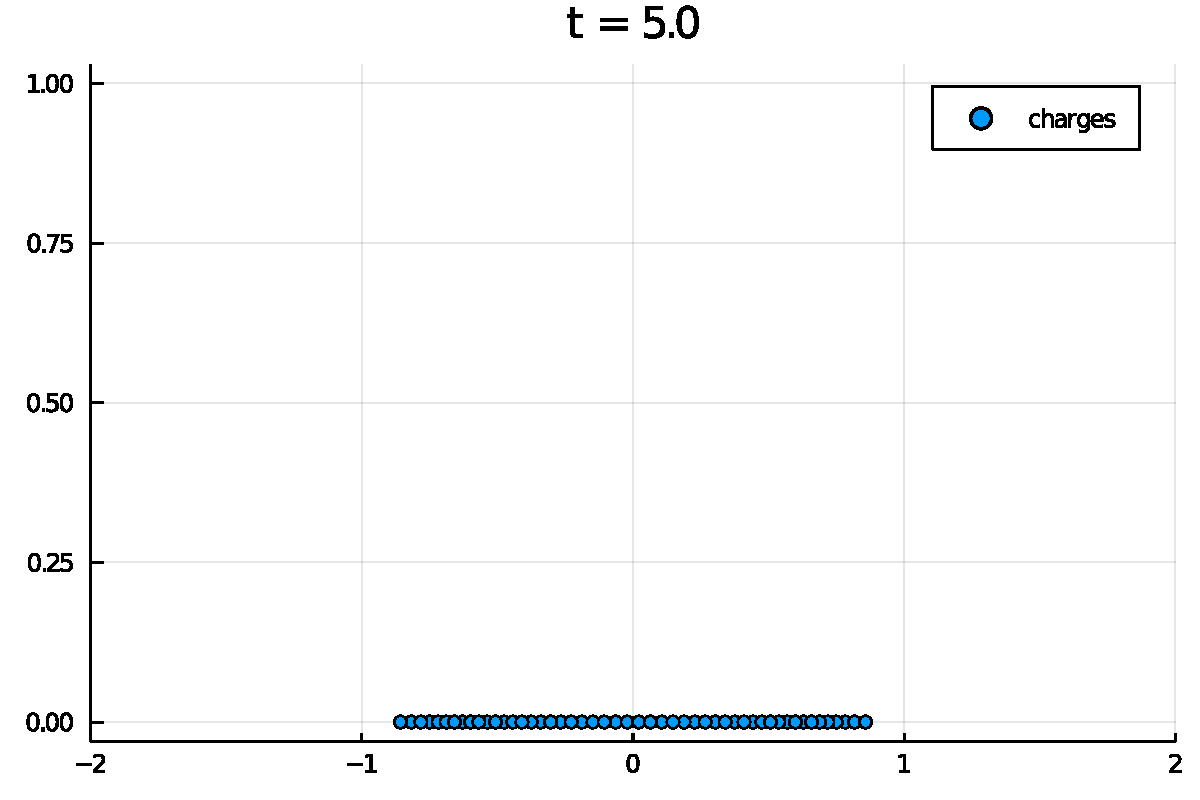
\includegraphics[width=\linewidth]{C:/Users/mfaso/OneDrive/Documents/GitHub/M3M6AppliedComplexAnalysis/output/figures/Solutions3_34_1.pdf}

The limiting distribution has the following form:


\begin{lstlisting}
(*@\HLJLnf{histogram}@*)(*@\HLJLp{(}@*)(*@\HLJLnf{\ensuremath{\lambda}}@*)(*@\HLJLp{(}@*)(*@\HLJLn{t}@*)(*@\HLJLp{)}@*)(*@\HLJLoB{/}@*)(*@\HLJLn{N}@*)(*@\HLJLoB{{\textasciicircum}}@*)(*@\HLJLp{(}@*)(*@\HLJLni{1}@*)(*@\HLJLoB{/}@*)(*@\HLJLni{4}@*)(*@\HLJLp{);}@*) (*@\HLJLn{nbins}@*)(*@\HLJLoB{=}@*)(*@\HLJLni{30}@*)(*@\HLJLp{,}@*) (*@\HLJLn{normalize}@*)(*@\HLJLoB{=}@*)(*@\HLJLkc{true}@*)(*@\HLJLp{,}@*) (*@\HLJLn{label}@*)(*@\HLJLoB{=}@*)(*@\HLJLs{"{}histogram}@*) (*@\HLJLs{of}@*) (*@\HLJLs{charges"{}}@*)(*@\HLJLp{)}@*)
\end{lstlisting}

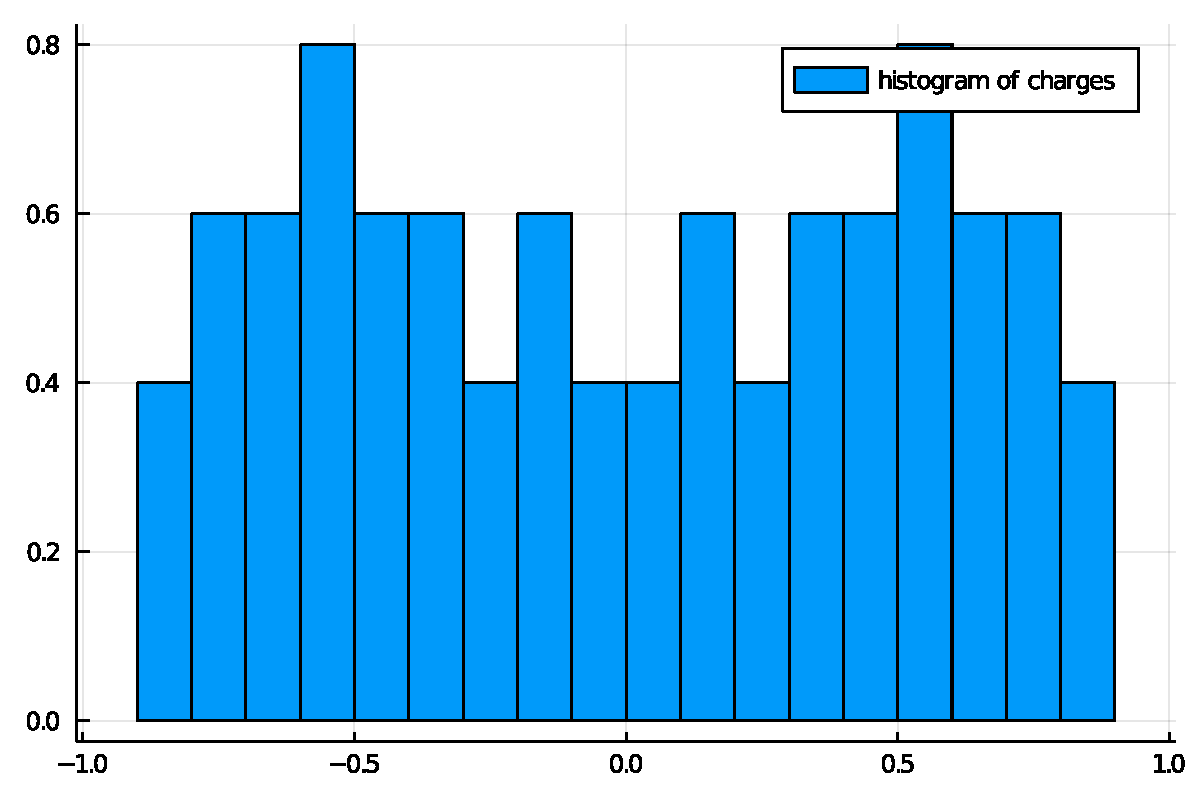
\includegraphics[width=\linewidth]{C:/Users/mfaso/OneDrive/Documents/GitHub/M3M6AppliedComplexAnalysis/output/figures/Solutions3_35_1.pdf}

We want to solve

\[
{\D^2 \lambda_k \over \D t^2} + \gamma {\D \lambda_k \over \D t} = \sum_{j=1 \atop j \neq k}^N {1 \over \lambda_k -\lambda_j} - 4\lambda_k^3
\]
Rescale via $\mu_k = {\lambda_k \over N^{1/4}}$ gives

\[
0 = N^{1/4} \br[{\D^2 \lambda_k \over \D t^2} + \gamma {\D \lambda_k \over \D t}] =
N^{-1/4} \sum_{j=1 \atop j \neq k}^N {1 \over \mu_k -\mu_j} - 4 N^{3/4} \mu_k^3
\]
or in other words

\[
0 = N^{-1/2} \br[{\D^2 \lambda_k \over \D t^2} + \gamma {\D \lambda_k \over \D t}] =
{1 \over N} \sum_{j=1 \atop j \neq k}^N {1 \over \mu_k -\mu_j} - 4 \mu_k^3
\]
We can now formally let $N\rightarrow \infty$ to get our equation

\[
\dashint_{-b}^b {w(t) \over x-t} \dt = 4 x^3
\]
where I've used symmetry to assume that the interval is symmetric. We want to find $w$ and $b$ so that this equations holds true and $w$ is a bounded probability density:

\begin{itemize}
\item[1. ] \[
w(x) >0
\]
for $-b < x < b$


\item[2. ] \[
\int w(x) \dx = 1
\]

\item[3. ] \[
w
\]
is bounded

\end{itemize}
Our equation is equivalent to

\[
\HH_{[-b,b]} w(x) = {4 x^3 \over \pi}
\]
recall the inversion formula

\[
    u(x) =  {-1 \over \sqrt{b^2 - x^2}}\HH \left[{ f(\diamond)  \sqrt{b^2-\diamond^2} }\right](x)  - {C \over \sqrt{b^2-x^2}}
\]
In our case $f(x) = {4 x^3 \over \pi}$ and we use

\[
\sqrt{z-b}\sqrt{z+b} = z\sqrt{1-b/z}\sqrt{1+b/z} = z - {b^2 \over 2 z} -{b^4 \over 8z^3} + O(z^{-4})
\]
to determine

\[
2 \I \CC \left[{ \diamond^3  \sqrt{b^2-\diamond^2} }\right](x) =
z^3(\sqrt{z-b}\sqrt{z+b} -z +  {b^2 \over 2 z} + {b^4 \over 8z^3}) = z^3\sqrt{z-b}\sqrt{z+b} -z^4 +  {b^2z^2 \over 2} + {b^4 \over 8}
\]

\begin{lstlisting}
(*@\HLJLn{b}@*) (*@\HLJLoB{=}@*) (*@\HLJLni{5}@*)
(*@\HLJLn{x}@*) (*@\HLJLoB{=}@*) (*@\HLJLnf{Fun}@*)(*@\HLJLp{(}@*)(*@\HLJLoB{-}@*)(*@\HLJLn{b}@*) (*@\HLJLoB{..}@*) (*@\HLJLn{b}@*)(*@\HLJLp{)}@*)
(*@\HLJLp{(}@*)(*@\HLJLni{2}@*)(*@\HLJLn{im}@*)(*@\HLJLp{)}@*)(*@\HLJLnf{cauchy}@*)(*@\HLJLp{(}@*)(*@\HLJLn{x}@*)(*@\HLJLoB{{\textasciicircum}}@*)(*@\HLJLni{3}@*)(*@\HLJLoB{*}@*)(*@\HLJLnf{sqrt}@*)(*@\HLJLp{(}@*)(*@\HLJLn{b}@*)(*@\HLJLoB{{\textasciicircum}}@*)(*@\HLJLni{2}@*)(*@\HLJLoB{-}@*)(*@\HLJLn{x}@*)(*@\HLJLoB{{\textasciicircum}}@*)(*@\HLJLni{2}@*)(*@\HLJLp{),}@*)(*@\HLJLn{z}@*)(*@\HLJLp{)}@*)
\end{lstlisting}

\begin{lstlisting}
71.6687198577313 + 40.090510492433154im
\end{lstlisting}


Therefore,


\begin{align*}
u(x) = {4\I \over \pi \sqrt{b^2 - x^2}}(\CC^+ + \CC^-) \left[{ \diamond^3  \sqrt{b^2-\diamond^2} }\right](x)  - {C \over \sqrt{b^2-x^2}} \\
{4 \over \pi \sqrt{b^2 - x^2}}(-x^4+{b^2 x^2 \over 2} + {b^4 \over 8})- {C \over \sqrt{b^2-x^2}}
\end{align*}
We choose $C$ so this is bounded, in particular, we get get the solution

\[
u(x) = {4 \over \pi \sqrt{b^2 - x^2}}(-x^4+{b^2 x^2 \over 2} + {b^4 \over 2})
\]

\begin{lstlisting}
(*@\HLJLn{u}@*) (*@\HLJLoB{=}@*) (*@\HLJLni{4}@*)(*@\HLJLoB{/}@*)(*@\HLJLp{(}@*)(*@\HLJLn{\ensuremath{\pi}}@*)(*@\HLJLoB{*}@*)(*@\HLJLnf{sqrt}@*)(*@\HLJLp{(}@*)(*@\HLJLn{b}@*)(*@\HLJLoB{{\textasciicircum}}@*)(*@\HLJLni{2}@*)(*@\HLJLoB{-}@*)(*@\HLJLn{x}@*)(*@\HLJLoB{{\textasciicircum}}@*)(*@\HLJLni{2}@*)(*@\HLJLp{))}@*)(*@\HLJLoB{*}@*)(*@\HLJLp{(}@*)(*@\HLJLoB{-}@*)(*@\HLJLn{x}@*)(*@\HLJLoB{{\textasciicircum}}@*)(*@\HLJLni{4}@*) (*@\HLJLoB{+}@*) (*@\HLJLn{b}@*)(*@\HLJLoB{{\textasciicircum}}@*)(*@\HLJLni{2}@*)(*@\HLJLoB{*}@*)(*@\HLJLn{x}@*)(*@\HLJLoB{{\textasciicircum}}@*)(*@\HLJLni{2}@*)(*@\HLJLoB{/}@*)(*@\HLJLni{2}@*) (*@\HLJLoB{+}@*) (*@\HLJLn{b}@*)(*@\HLJLoB{{\textasciicircum}}@*)(*@\HLJLni{4}@*)(*@\HLJLoB{/}@*)(*@\HLJLni{2}@*)(*@\HLJLp{)}@*)
(*@\HLJLnf{H}@*)(*@\HLJLp{(}@*)(*@\HLJLn{u}@*)(*@\HLJLp{,}@*) (*@\HLJLnfB{0.1}@*)(*@\HLJLp{),}@*)(*@\HLJLni{4}@*)(*@\HLJLoB{*}@*)(*@\HLJLnfB{0.1}@*)(*@\HLJLoB{{\textasciicircum}}@*)(*@\HLJLni{3}@*)(*@\HLJLoB{/}@*)(*@\HLJLn{\ensuremath{\pi}}@*)
\end{lstlisting}

\begin{lstlisting}
(0.0012732395447351292, 0.001273239544735163)
\end{lstlisting}


At least it looks right, we just need to get the right b:


\begin{lstlisting}
(*@\HLJLnf{plot}@*)(*@\HLJLp{(}@*)(*@\HLJLn{u}@*)(*@\HLJLp{;}@*) (*@\HLJLn{label}@*) (*@\HLJLoB{=}@*) (*@\HLJLs{"{}b}@*) (*@\HLJLs{=}@*) (*@\HLJLsi{{\$}b}@*)(*@\HLJLs{"{}}@*)(*@\HLJLp{)}@*)
\end{lstlisting}

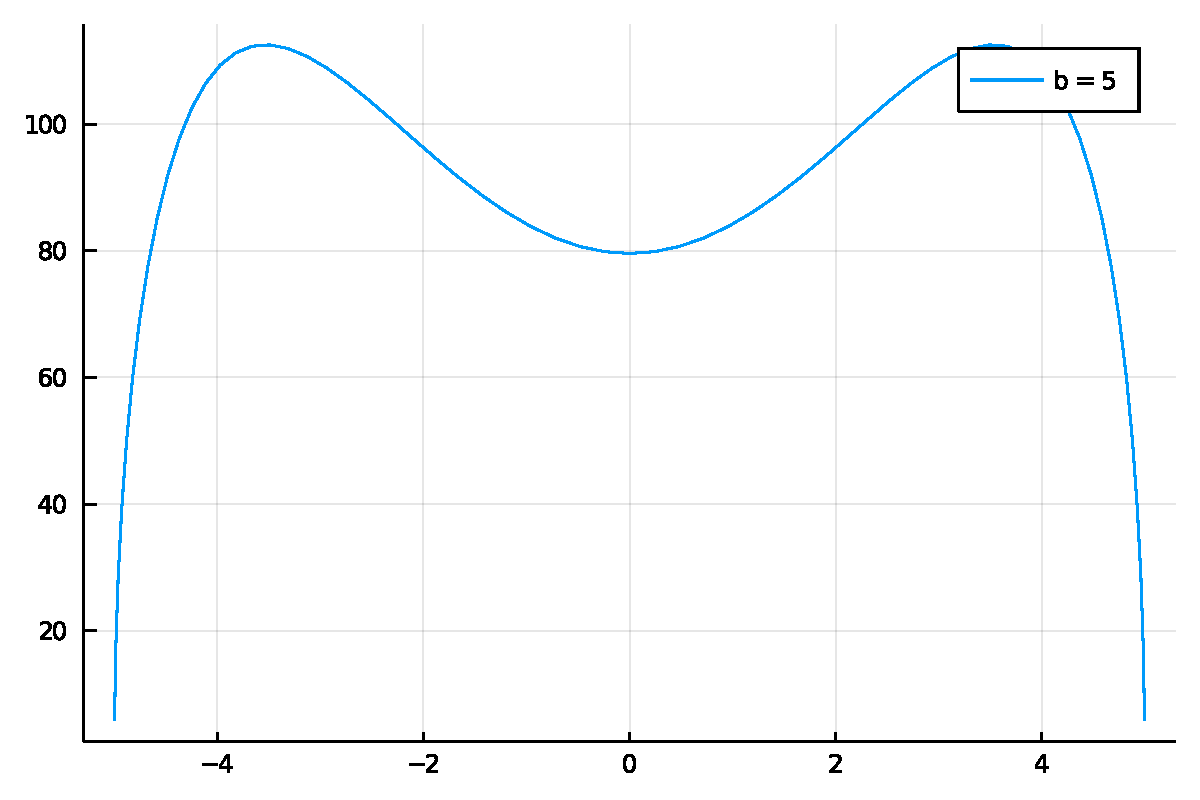
\includegraphics[width=\linewidth]{C:/Users/mfaso/OneDrive/Documents/GitHub/M3M6AppliedComplexAnalysis/output/figures/Solutions3_38_1.pdf}

We want to choose $b$ now so that this integrates to $1$. For example, this choice of $b$ is horrible:


\begin{lstlisting}
(*@\HLJLnf{sum}@*)(*@\HLJLp{(}@*)(*@\HLJLn{u}@*)(*@\HLJLp{)}@*)
\end{lstlisting}

\begin{lstlisting}
937.5
\end{lstlisting}


There's a nice trick: If $-2\pi \I \CC u(z) \sim {1 \over  z}$ then $\int_{-b}^b u(x) \dx  = 1$.  We know since

\[
{1 \over \sqrt{1+z}} = 1 - {z \over 2} + {3z^2 \over 8} - {5z^3 \over 16} + O(z^4)
\]

\begin{align*}
 {-z^4 +  {b^2z^2 \over 2} + {b^4 \over 2} \over \sqrt{z-b}\sqrt{z+b}} &=  {-z^3 +  {b^2z \over 2} + {b^4 \over 2 z} \over \sqrt{1-b/z}\sqrt{1+b/z}} \\
 &=  (-z^3 +  {b^2z \over 2} )(1 + {b \over 2 z} + {3 b^2 \over 8 z^2} + {5 b^3 \over 16z^3} )(1 - {b \over 2 z} + {3 b^2 \over 8 z^2}  - {5 b^3 \over 16z^3}) + O(z^{-1}) \\
 &=-z^3  + \pr({b^2  \over 2} +{b^2 \over 4} + {b^2 \over 2} - {3 b^2 \over 8} -{3 b^2 \over 8} ) z +O(z^{-1})\\
 &= -z^3 + O(z^{-1})
 \end{align*}
Thus we know

\[
\CC  u(z) = {2\I \over \pi} z^3 +{2 \I \over \pi} {-z^4 +  {b^2z^2 \over 2} + {b^4 \over 2} \over \sqrt{z-b}\sqrt{z+b}}
\]

\begin{lstlisting}
(*@\HLJLnf{cauchy}@*)(*@\HLJLp{(}@*)(*@\HLJLn{u}@*)(*@\HLJLp{,}@*) (*@\HLJLn{z}@*)(*@\HLJLp{)}@*)

(*@\HLJLn{z}@*) (*@\HLJLoB{=}@*)(*@\HLJLnfB{100.0}@*)(*@\HLJLn{im}@*)(*@\HLJLp{;}@*)
(*@\HLJLni{2}@*)(*@\HLJLn{im}@*)(*@\HLJLoB{/}@*)(*@\HLJLn{\ensuremath{\pi}}@*)(*@\HLJLoB{*}@*)(*@\HLJLn{z}@*)(*@\HLJLoB{{\textasciicircum}}@*)(*@\HLJLni{3}@*) (*@\HLJLoB{+}@*) (*@\HLJLni{2}@*)(*@\HLJLn{im}@*)(*@\HLJLoB{/}@*)(*@\HLJLn{\ensuremath{\pi}}@*)(*@\HLJLoB{*}@*)(*@\HLJLp{(}@*)(*@\HLJLoB{-}@*)(*@\HLJLn{z}@*)(*@\HLJLoB{{\textasciicircum}}@*)(*@\HLJLni{4}@*) (*@\HLJLoB{+}@*) (*@\HLJLn{b}@*)(*@\HLJLoB{{\textasciicircum}}@*)(*@\HLJLni{2}@*)(*@\HLJLoB{*}@*)(*@\HLJLn{z}@*)(*@\HLJLoB{{\textasciicircum}}@*)(*@\HLJLni{2}@*)(*@\HLJLoB{/}@*)(*@\HLJLni{2}@*) (*@\HLJLoB{+}@*)(*@\HLJLn{b}@*)(*@\HLJLoB{{\textasciicircum}}@*)(*@\HLJLni{4}@*)(*@\HLJLoB{/}@*)(*@\HLJLni{2}@*)(*@\HLJLp{)}@*)(*@\HLJLoB{/}@*)(*@\HLJLp{(}@*)(*@\HLJLnf{sqrt}@*)(*@\HLJLp{(}@*)(*@\HLJLn{z}@*)(*@\HLJLoB{-}@*)(*@\HLJLn{b}@*)(*@\HLJLp{)}@*)(*@\HLJLnf{sqrt}@*)(*@\HLJLp{(}@*)(*@\HLJLn{z}@*)(*@\HLJLoB{+}@*)(*@\HLJLn{b}@*)(*@\HLJLp{))}@*)
\end{lstlisting}

\begin{lstlisting}
1.4908359390683472 - 0.0im
\end{lstlisting}


taking this one term further we find

\[
 {-z^4 +  {b^2z^2 \over 2} + {b^4 \over 2} \over \sqrt{z-b}\sqrt{z+b}} = -z^3 +{3 b^4 \over 8 z} + O(z^{-2})
\]
Hence we want to choose $b$ so that

\[
-2\I\pi \CC u(z) = {3 b^4 \over 2 z} \sim {1 \over z}
\]
in other words, $b = ({2 \over 3})^{1/4}$


\begin{lstlisting}
(*@\HLJLn{b}@*) (*@\HLJLoB{=}@*) (*@\HLJLp{(}@*)(*@\HLJLni{2}@*)(*@\HLJLoB{/}@*)(*@\HLJLni{3}@*)(*@\HLJLp{)}@*)(*@\HLJLoB{{\textasciicircum}}@*)(*@\HLJLp{(}@*)(*@\HLJLni{1}@*)(*@\HLJLoB{/}@*)(*@\HLJLni{4}@*)(*@\HLJLp{)}@*)
(*@\HLJLn{x}@*) (*@\HLJLoB{=}@*) (*@\HLJLnf{Fun}@*)(*@\HLJLp{(}@*)(*@\HLJLoB{-}@*)(*@\HLJLn{b}@*) (*@\HLJLoB{..}@*) (*@\HLJLn{b}@*)(*@\HLJLp{)}@*)
(*@\HLJLn{u}@*) (*@\HLJLoB{=}@*) (*@\HLJLni{4}@*)(*@\HLJLoB{/}@*)(*@\HLJLp{(}@*)(*@\HLJLn{\ensuremath{\pi}}@*)(*@\HLJLoB{*}@*)(*@\HLJLnf{sqrt}@*)(*@\HLJLp{(}@*)(*@\HLJLn{b}@*)(*@\HLJLoB{{\textasciicircum}}@*)(*@\HLJLni{2}@*)(*@\HLJLoB{-}@*)(*@\HLJLn{x}@*)(*@\HLJLoB{{\textasciicircum}}@*)(*@\HLJLni{2}@*)(*@\HLJLp{))}@*)(*@\HLJLoB{*}@*)(*@\HLJLp{(}@*)(*@\HLJLoB{-}@*)(*@\HLJLn{x}@*)(*@\HLJLoB{{\textasciicircum}}@*)(*@\HLJLni{4}@*) (*@\HLJLoB{+}@*) (*@\HLJLn{b}@*)(*@\HLJLoB{{\textasciicircum}}@*)(*@\HLJLni{2}@*)(*@\HLJLoB{*}@*)(*@\HLJLn{x}@*)(*@\HLJLoB{{\textasciicircum}}@*)(*@\HLJLni{2}@*)(*@\HLJLoB{/}@*)(*@\HLJLni{2}@*) (*@\HLJLoB{+}@*) (*@\HLJLn{b}@*)(*@\HLJLoB{{\textasciicircum}}@*)(*@\HLJLni{4}@*)(*@\HLJLoB{/}@*)(*@\HLJLni{2}@*)(*@\HLJLp{)}@*)
(*@\HLJLnf{sum}@*)(*@\HLJLp{(}@*)(*@\HLJLn{u}@*)(*@\HLJLp{)}@*)
\end{lstlisting}

\begin{lstlisting}
0.9999999999999997
\end{lstlisting}


And it worked!


\begin{lstlisting}
(*@\HLJLnf{histogram}@*)(*@\HLJLp{(}@*)(*@\HLJLnf{\ensuremath{\lambda}}@*)(*@\HLJLp{(}@*)(*@\HLJLnfB{5.0}@*)(*@\HLJLp{)}@*)(*@\HLJLoB{/}@*)(*@\HLJLn{N}@*)(*@\HLJLoB{{\textasciicircum}}@*)(*@\HLJLp{(}@*)(*@\HLJLni{1}@*)(*@\HLJLoB{/}@*)(*@\HLJLni{4}@*)(*@\HLJLp{);}@*) (*@\HLJLn{nbins}@*)(*@\HLJLoB{=}@*)(*@\HLJLni{25}@*)(*@\HLJLp{,}@*) (*@\HLJLn{normalize}@*)(*@\HLJLoB{=}@*)(*@\HLJLkc{true}@*)(*@\HLJLp{,}@*) (*@\HLJLn{label}@*)(*@\HLJLoB{=}@*)(*@\HLJLs{"{}histogram}@*) (*@\HLJLs{of}@*) (*@\HLJLs{charges"{}}@*)(*@\HLJLp{)}@*)
(*@\HLJLnf{plot!}@*)(*@\HLJLp{(}@*)(*@\HLJLn{u}@*)(*@\HLJLp{;}@*) (*@\HLJLn{label}@*)(*@\HLJLoB{=}@*)(*@\HLJLs{"{}u"{}}@*)(*@\HLJLp{,}@*)(*@\HLJLn{xlims}@*)(*@\HLJLoB{=}@*)(*@\HLJLp{(}@*)(*@\HLJLoB{-}@*)(*@\HLJLni{2}@*)(*@\HLJLp{,}@*)(*@\HLJLni{2}@*)(*@\HLJLp{))}@*)
\end{lstlisting}

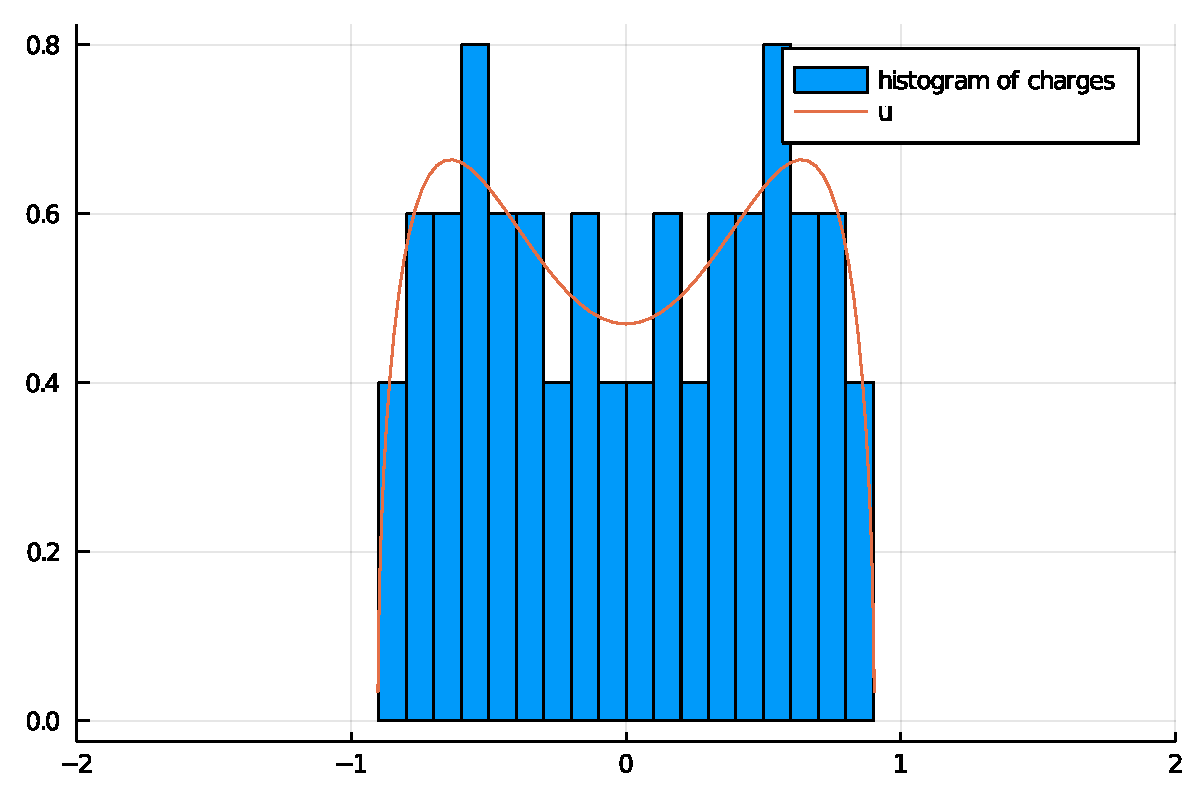
\includegraphics[width=\linewidth]{C:/Users/mfaso/OneDrive/Documents/GitHub/M3M6AppliedComplexAnalysis/output/figures/Solutions3_42_1.pdf}

}
\end{document}
